
\documentclass [twoside,openbib,12pt]{article}
\usepackage{epsfig}
\usepackage{graphicx}
\usepackage{amsmath}
\usepackage[titletoc]{appendix}
\usepackage{enumitem}

%\usepackage{draftwatermark}
%\SetWatermarkText{DRAFT}
%\SetWatermarkScale{6}
%\usepackage[printwatermark]{xwatermark}
%\newwatermark*[allpages,angle=45,scale=5,xpos=0,ypos=0]{DRAFT}

\usepackage{tikz}
\usepackage[printwatermark]{xwatermark}
\newsavebox\mybox
\savebox\mybox{\tikz[color=red,opacity=0.3]\node{\bfseries\sffamily DRAFT};}
\newwatermark*[allpages,angle=45,scale=8,xpos=-25,ypos=20
]{\usebox\mybox}

% These commands are to set up the page, and should be self-evident

\evensidemargin 0.0 mm
\oddsidemargin 0.0 mm

\voffset -15 mm
\textwidth 170 mm

\textheight 230 mm
\headsep 0.0 mm
\usepackage[figuresleft]{rotating}
\usepackage[bookmarks=true]{hyperref}

%some shorthands
\newcommand{\bmath}{\begin{displaymath}}
\newcommand{\emath}{\end{displaymath}}

\newcommand{\beq}{\begin{equation}}
\newcommand{\eeq}{\end{equation}}
\newcommand{\bea}{\begin{eqnarray}}
\newcommand{\eea}{\end{eqnarray}}

\newcommand{\bfg}{\begin{figure}}
\newcommand{\efg}{\end{figure}}
\newcommand{\bitm}{\begin{itemize}}
\newcommand{\eitm}{\end{itemize}}
\newcommand{\bnum}{\begin{enumerate}}
\newcommand{\enum}{\end{enumerate}}
\newcommand{\btbl}{\begin{table}}
\newcommand{\etbl}{\end{table}}
\newcommand{\btbu}{\begin{tabular}}
\newcommand{\etbu}{\end{tabular}}

\newcommand{\ra}{\rightarrow}
\newcommand{\Ra}{\Rightarrow}
%these can also be put into a separate file so that one doesn't need to paste them into every tex file

%\include{def_com}
%%%%%%%%%%%%%%%----------------------------------


\begin{document}
\normalsize
\parskip=5pt plus 1pt minus 1pt

\title{ \hfill\parbox{4cm}{\normalsize
                          \hbox{Document-34898          \hfill}
                          \hbox{Bo Xin          \hfill}
                          \hbox{Doug Neil         \hfill}
                          \hbox{Sandrine Thomas          \hfill}
                           \hbox{For the LSST M1M3 Team          \hfill}
                          \hbox{\today             \hfill}}\\[1cm]
{\bf
M1M3 Optical Testing Results at the UofA Mirror Lab
}
}
\author{}
\date{}

\maketitle
%\newpage
\begin{abstract}
  The M1M3 optical testing at the University of Arizona 
  (UofA) Richard F. Caris Mirror Lab has
  been very successful.
This document describes the analysis results from those testing campaigns.
\end{abstract}

%if you need a table of content
\tableofcontents

%\renewcommand{\thesection}{\arabic{section}}\setcounter{section}{-1}

\section{Introduction}
\label{sec:intro}

In January and Feburary 2019, the fully assembled M1M3 system, with
the glass mirror on top of the mirror cell, modulo the thermal control
system, underwent actuated test at the UofA Mirror Lab.
The testing consisted of two testing campaigns, each lasted
approximately two weeks.
First campaign from 1/14 to 1/25, minus Monday 1/21 which was MLK day.
The second from 2/11 to 2/22, minus Friday 2/22 which was Rodeo day.
In this document, we describe the analysis results from those testing
campaigns.

The main objectives of the testing campaigns were two-fold:
(1) optimizing the M1M3 surface, with optimized support forces, and
(2) characterizing how the surface responds to actuator forces,
including measuring the bending modes and single actuator influence functions.
Both main objectives were successfully achieved.
Of course, during the process, we exercised the control software, and
the hardware, learned a lot about the as-built system, and came up with a long list of items that could be
further improved, as summarized by Doug Neil in his lessons-learned document.
But those are not the major topic for this document.
We will just say that the entire software plus hardware system have
been very robust.
They worked for the entire testing campaigns, without
any glitches, and without being powered down.
The only exception is the Engineering Facility Database (EFD), which
we will discuss in my detail in Section~\ref{sec:efd}.
Everything has been very
repeatible, as we will see from some analysis results we will present
later in this document.

The analysis has been done in Python notebooks, and documented on
GitHub \url{https://github.com/bxin/M1M3_ML}.
The only exception is that some of the real-time analysis, where fast
turn-around was needed, was done in Matlab. This is because most of
the analysis done at the M1M3 acceptance, described in document-17171~\cite{m1m3perf},
was done in Matlab.
The notebooks provide both a day-by-day accounting of what was done, i.e.,
what results were obtained on each day, why we did what we did, and some more targeted
analysis, including tutorials.
Other than holidays, there is no notebook for 1/23 because on that day
the Mirror Lab crew performed CGH calibration and worked on
empirical force analysis for fixing the divits above the quads.
A summary of what tests have been performed for each of the major
tasks can be found in summary\_by\_task.txt in the GitHub repo. 

Other useful background information relevant to the testing include
\bitm
\item UofA test plan~\cite{m1m3UAtestplan}
\item  Data analysis plan presented at M1M3 Optical Test Readiness
  Review~\cite{m1m3anaplan}
\item Data processing precedure description~\cite{m1m3processing}
\item M1M3 performance analysis at mirror acceptance (2015)~\cite{m1m3perf}.
\eitm
Note that the Mirror Lab also produced a data analysis report for
these testing campaigns~\cite{m1m3UAreport}. What we describe here in this document is
complimentary to the Mirror Lab report.
We do not want to duplicate work. 
It should be noted that in a lot of cases, where we have examined the
Mirror Lab data processing and analysis in detail, and felt that we
understand everything, we simply use their results, or refer to
figures and tables in their report directly.
As one can see from the Python notebooks, in those cases, we simply
read the Mirror Lab analysis output from the data packages they provided.

In the rest of this document (Sections~\ref{sec:ab} through \ref{sec:horizon}), we will describe each major task in a
separate section. We follow the order as outlined in
summary\_by\_task.txt in the above GitHub repo.
Section~\ref{sec:ferror}, the actuator force error analysis, was not a
major task as listed in the test plan.
But with all the data we collected it came for free.
It should be noted that the order the tasks and results are described
in this document does not reflect the order the tests were carried out
during the testing.
The order the tests were executed in the Mirror Lab had to take into
account practicality, to make sure things run smoothly and efficiently.

Note that most of the measurements we took were differential
measurements, i.e., we were more interested in the differences between
subsequent measurements, rather than individual
measurements. Measurements were always taken a quickly as possible, to
avoid thermal drifts, which could invalidate differential measurements.
Thermal corrections are not included in most of the data processing.

\section{Coordinate System Definition}

Before doing any quantitative analysis, it is important to make sure
we have a clear definition of the coordinate
system. Figure.~\ref{fig:cs} shows the layout of the 156
actuators, as in the M1M3 optical coordinate system.
This
is looking at the M1M3 surface from M2.
This will be the standard coordinate system we use for all the
analysis presented in this document.
The mirror cell access door is at the $+y$ position.
In the Mirror Lab, the $x$-axis pointed toward the control station.


  \begin{figure}[bthp]
   \begin{center}
   \begin{tabular}{c}
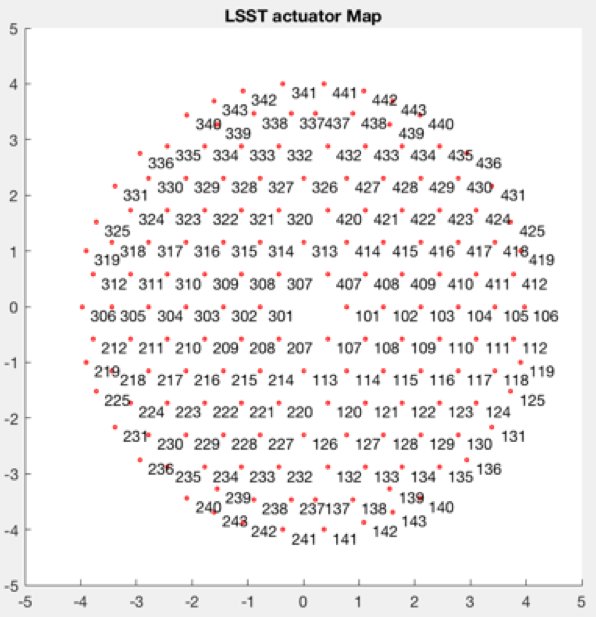
\includegraphics[width=100mm]{figures/cs.png}
  \end{tabular}
   \end{center}
   \caption
  { \label{fig:cs}
M1M3 actuator ID numbers in the M1M3 optical coordinate system. This
is looking at the M1M3 surface from M2. This will be the standard coordinate system we use for all the
analysis presented in this document.
 }
\end{figure}

We note that most of the LSST engineering drawings use a different
coordinate system, as shown in Figure~\ref{fig:actMap}.
The $y$ axis is the same as the M1M3 optical coordinate system, but
the $x$ axis is flipped.
The mirror cell access door is still at the $+y$ position.
In the Mirror Lab, the $x$-axis pointed away from the control station.
This is more intuitive when one works inside the mirror cell, for
example, while installing the actuators.

Figure~\ref{fig:actMap} also shows the actuator
 ID numbers and their types.
The actuator types indicate whether it is a single-axis actuator (SAA)
or dual-axis actuator (DAA), the orientation of the secondary
cylinder, which is also indicated by the arrows in
Figure.~\ref{fig:actMap}, and the number of pucks for each
load-spreader.
The index keys can be found in \url{https://github.com/bxin/M1M3_ML/blob/master/data/LS_CUP_ACTSTYLE_ID.xlsx}.

  \begin{figure}[bthp]
   \begin{center}
   \begin{tabular}{c}
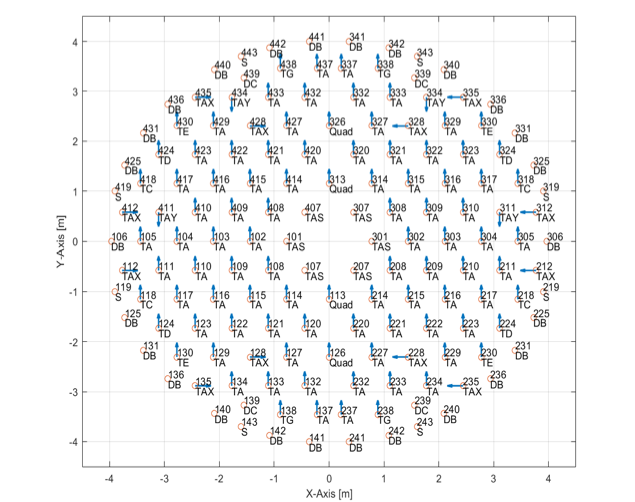
\includegraphics[width=140mm]{figures/actMap.png}
  \end{tabular}
   \end{center}
   \caption
  { \label{fig:actMap}
M1M3 actuator ID numbers, types, and their locations while looking at the mirror from inside the cell.
 }
\end{figure}

Before any tests began, we verified with the Mirror Lab that we were
using the same coordinate system, and the $x$ and $y$ coordinates of
the actuators all agree.

\section{Optimize Measurement Parameters}
\label{sec:ab}

\subsection{Number of samples and time interval for each measurement}

Due to instabilities in the testing hardware, mostly from air
turbulence in the optical path and hardware vibration,
each surface measurement is an average
of many samples. A sample itself is the average of a series of short
exposures, where the averaging is done automatically by the 4D
software that came with the interferometer. The number of samples for
each surface measurement, and the time interval between the samples,
are configurable parameters.
We use the shorthand $a\times bs$ for $a$ samples separated by $b$ seconds.
Before we start taking measurements to characterize the mirror bending
properties and optimizing the mirror surfaces, we need to optimize $a$
and $b$.

To determine $a$ and $b$, we tested three configurations, each taking
an equal amount of time to acquire:
\bnum
\item $10 \times 5$s
\item $5 \times 10$s
\item $25 \times 2$s
\enum
We did this for M1 only. For each configuration, we took 4
measurements.
For each measurement, we take the average of all the samples, $s1$,
$s2$, $s3$, $s4$ (we call these sub-averages), then average the 4 measurements, $s =
(s1+s2+s3+s4)/4$.
The sub-averages for the $25 \times 2s$ configuration is
shown in Figure~\ref{fig:ab}.

  \begin{figure}[bthp]
   \begin{center}
   \begin{tabular}{c}
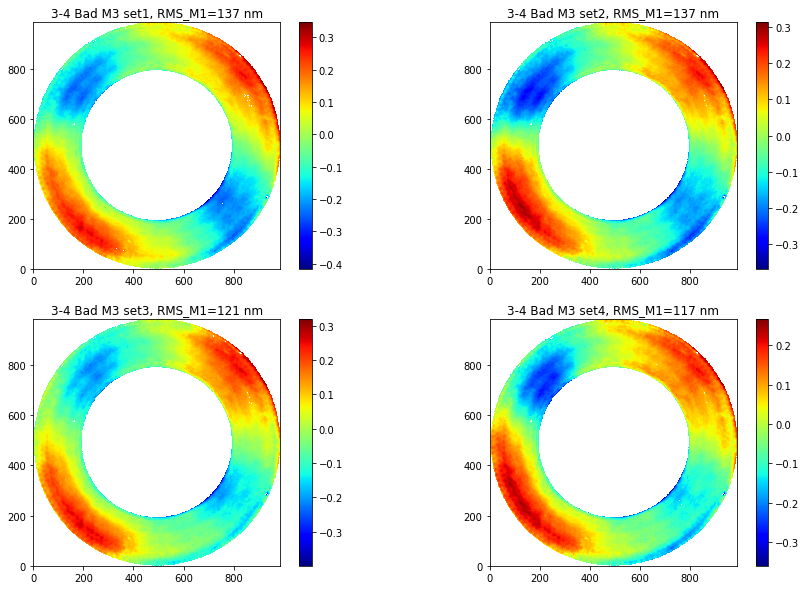
\includegraphics[width=150mm]{figures/ab25x2.png}
  \end{tabular}
   \end{center}
   \caption
  { \label{fig:ab}
M1 surface maps sub-averages with the $25 \times 2s$ configuration.
 }
\end{figure}

The RMS of the difference maps between these sub-averages shown in Figure~\ref{fig:ab} and their
grand-average ($s$) is calculated to be 24 nm.
For comparison, the same RMS values for the $10 \times 5$s and $5
\times 10$s configurations are found to be 28 nm.
As another check, we also repeated this test with a $40 \times 5$s
configuration. With much longer averaging time, the RMS difference
between the sub-averages and the grand-average remained at 24 nm.
We therefore concluded that the $25 \times 2s$ configuration is very
close to optimal, and decided to use that for all subsequent
measurements.

The analysis in Jupyter Notebook format is found at
\url{https://github.com/bxin/M1M3_ML/blob/master/190115.ipynb}

\subsection{Number of measurements for averaging}

To determine the number of measurements needed for averaging, we took
10 M1 measurements, then 20 M3 measurements, then another 10 M1
measurements.
For the analysis part, we sub-divide these 20 M1 and 20 M3 measurement
into groups of 2, 5, and 10 measurements. Within each group, we
calculated the group sub-averages, and the grand-average of all the
measurements.
The idea is that the grand-averages can be used as the ``truth'', and
we calculate the RMS differences between the sub-averages and the grand-averages.
Note that the average of the first 10 M1 measurements
was seen to be very different from the second 10 M1 measurements, so
we had to use 2 grand-averages for M1. 

The criteria was that we want the noise on the surface measurements in
RMS to be less than 20 nm. This corresponds to the non-repeatible
error in the surface measurements. With the initial acceptance
testing, we got the RMS error on both surfaces below 20 nm. Note that
the as-built M1M3 surface, as measured during M1M3 acceptance testing,
contributes to 120 mas in PSF FWHM, including 104 mas from M1 and 60
mas from M3~\cite{m1m3perf}. The total error budget allocated to the as-built LSST
system is 400 mas.

We refer the reader to Figures
1 and 2 of the Mirror Lab analysis report~\cite{m1m3UAreport}
for the RMS differences
versus the number of measurements in groups.
As can be seen there, for M3, things converge pretty quickly. We only
need one measurement for M3. We could even shorten each M3 measurement
to be $20 \times 2s$ without sacrificing much measurement accuracy.
For M1, 2 measurements, each of $25 \times 2s$, would be needed.
So from this point on, we define each M1 measurement as $50 \times
2s$, and each M3 measurement as $20 \times 2s$.
As the result, for the bending modes and influence function
measurements, M1 took much longer than M3.

We want the measurements to be long enough to average out the
fast-changing factors, such as the air turbulence. Meanwhile we do not
want an individual measurement to take too long, because thermal
conditions would be slowly drifting.


The analysis in Jupyter Notebook format is found at
\url{https://github.com/bxin/M1M3_ML/blob/master/190115.ipynb}

\section{Repeatability Tests}

We did a lot of repeatability tests, which we discuss in detail
next. This involved adding additional forces to the actuators to
produce a low-order or high-order bending mode, then removing it, or
translating the mirror using the hard points then translating back, etc.
At the end of the operations, we remeasure the mirror surfaces, and see
how much has changed in surface measurements.

We assumed that M1 is more sensitive to perturbations, due to its
larger diameter.
For most of these repeatability tests,
we measured M1 only. For the test where we removed an actuator then
reinstalled it, we measured both M1 and M3, as some actuators removed were
under M3.

Right before these tests, we measured the reference surfaces , which is shown in
Figure~\ref{fig:repeatRef}.
The reference forces were one of the force sets obtained during the
early optimization process.
It doesn't matter what exact forces we use, as long as they give a
good measurable surface. We are only interested in the differences
between measurements.

 \begin{figure}[bthp]
   \begin{center}
   \begin{tabular}{c}
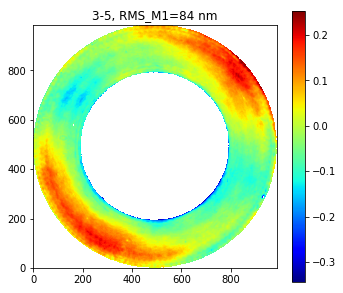
\includegraphics[width=60mm]{figures/repeatRef.png}
  \end{tabular}
   \end{center}
   \caption
  { \label{fig:repeatRef}
M1 reference surface before the repeatability tests.
 }
\end{figure}


Most of the analysis described in this section is found at
\url{https://github.com/bxin/M1M3_ML/blob/master/190116.ipynb}
The only exception is that the removing and reinstalling actuator part
is in
\url{https://github.com/bxin/M1M3_ML/blob/master/190221.ipynb}

\subsection{Add low-order bending mode, then remove it}
\label{sec:repeatB1}

For low order bending modes, a small amount of forces produce a
relatively large surface deformation, measured by the surface
RMS. When applying bending modes to introduce surface deformations
during the testing, based on the Mirror Lab experience, a general rule of thumb is that a surface RMS of
about 500 nm or below is desirable. This is large enough for it to be seen by
the interferometer, but not too large to cause confusion in
interpreting the fringes.

Based on the 500 nm rule,
we applied 3N of RMS forces to produce bending mode No. 1, which is
one of the two astigmatism modes, then removed it, then remeasured the
M1 surface. Figure.~\ref{fig:repeatB1} shows the new map, as well as the
difference from the reference map. The RMS of the difference map is 20
nm, which is on the same level as the measurement accuracy.

 \begin{figure}[bthp]
   \begin{center}
   \begin{tabular}{c}
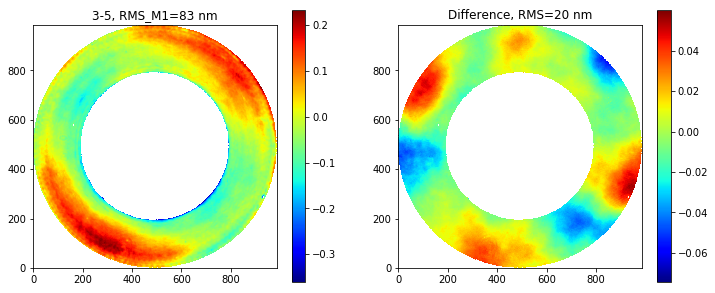
\includegraphics[width=120mm]{figures/repeatB1.png}
  \end{tabular}
   \end{center}
   \caption
  { \label{fig:repeatB1}
Measured M1 surface after we added 3N of bending mode No. 1 then
removed it (left), and the difference from the reference map
(right). The reference map is shown in Figure.~\ref{fig:repeatRef}.
 }
\end{figure}

\subsection{Add high-order bending mode, then remove it}

Repeating the procedure as described in Section.~\ref{sec:repeatB1}
with a high order bending mode, 20N RMS of No. 22 in this case, gave
us results shown in Figure.~\ref{fig:repeatB22}. 
The RMS of the difference map is 17
nm, which is on the same level as the measurement accuracy.

Repeating the procedure with 40N and 60N RMS of bending mode No. 22
gave very similar results. The RMS of the resulting difference maps
were 14 nm and 18 nm, respectively, in those two cases.

 \begin{figure}[bthp]
   \begin{center}
   \begin{tabular}{c}
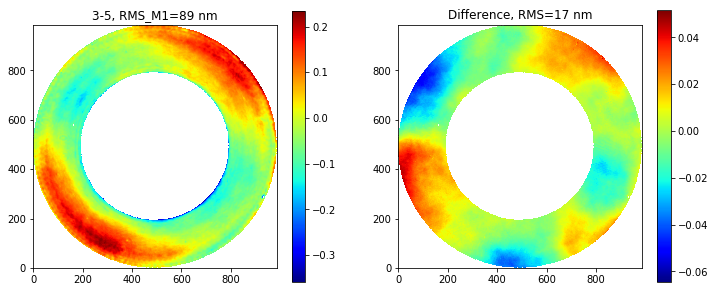
\includegraphics[width=120mm]{figures/repeatB22.png}
  \end{tabular}
   \end{center}
   \caption
  { \label{fig:repeatB22}
Measured M1 surface after we added 20N of bending mode No. 22 then
removed it (left), and the difference from the reference map
(right). The reference map is shown in Figure.~\ref{fig:repeatB1} (left).
 }
\end{figure}

\subsection{Translate the mirror, then back}

Next, we repositioned the mirror using the hard points, specifically,
by translating the mirror 1 mm along $+x$ axis, then translate it
back, and remeasure the M1 surface. We also repeated this procedure
for $+y$ and $+z$ directions. As the example, results for $+x$
translation is given in Figure.~\ref{fig:repeatX}.
The resulting RMS of the difference maps are 17, 17, and 33
nm, for the x, y, and z translations, respectively.

 \begin{figure}[bthp]
   \begin{center}
   \begin{tabular}{c}
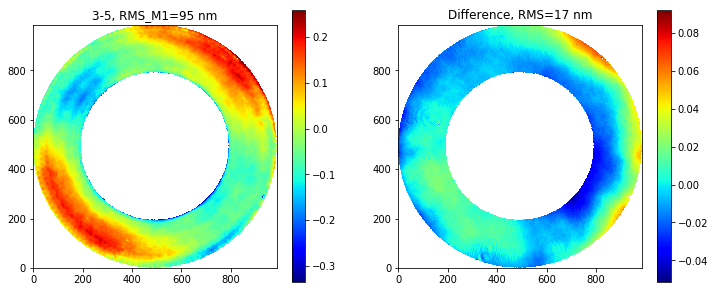
\includegraphics[width=120mm]{figures/repeatX.png}
  \end{tabular}
   \end{center}
   \caption
  { \label{fig:repeatX}
Measured M1 surface after we translated the mirror along $+x$
direction by 1mm, then moved it back (left), and the difference from the reference map
(right). The reference map here is the M1 map after we removed the 60
N RMS of bending mode No. 22.
 }
\end{figure}


\subsection{Lower the mirror, then raise it}

We then lowered the mirror onto its static supports, then raised it,
reapplied the nominal forces, 
then remeasured M1 surface. 
The observed RMS difference was 39 nm, as shown in Figure~\ref{fig:lowerRaise}.

 \begin{figure}[bthp]
   \begin{center}
   \begin{tabular}{c}
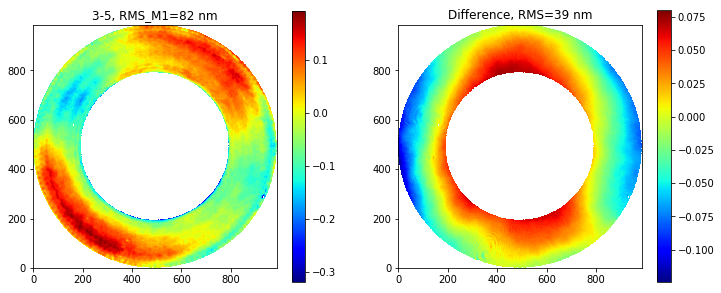
\includegraphics[width=120mm]{figures/lowerRaise.png}
  \end{tabular}
   \end{center}
   \caption
  { \label{fig:lowerRaise}
Measured M1 surface after we lowered, then raised the mirror (left), and the difference from the reference map
(right). The reference map is the M1 map after we moved the mirror
back to nominal position after the 1 mm $+z$ translation.
 }
\end{figure}

\subsection{Remove an actuator, then reinstall it}

Because the mirror would need to be detached from the cell before the
two being shipped to Chile separately, we wanted to understand better
how repeatible the actuator installations are.

To do this test, we picked four actuators, with ID numbers 337, 114, 113, 411, representing different
actuator types and various locations.
We removed and re-installed each actuator one after another, and
measured surfaces in between this process.
For example, we first take a M1-M3-M1 reference measurement, then
removed actuator 337, followed by a reinstallation of actuator
337. Then we take the second M1-M3-M3 measurement.

There were a total of five surface measurements, before and after
removing and reinstalling the four actuators.
The five surface measurements are shown in Figure~\ref{fig:reinstall}.
The four difference maps are shown in Figure~\ref{fig:reinstallDiff}.
The RMS values of all the surface measurements as well as the
different maps are shown on plot titles.

 \begin{figure}[bthp]
   \begin{center}
   \begin{tabular}{c}
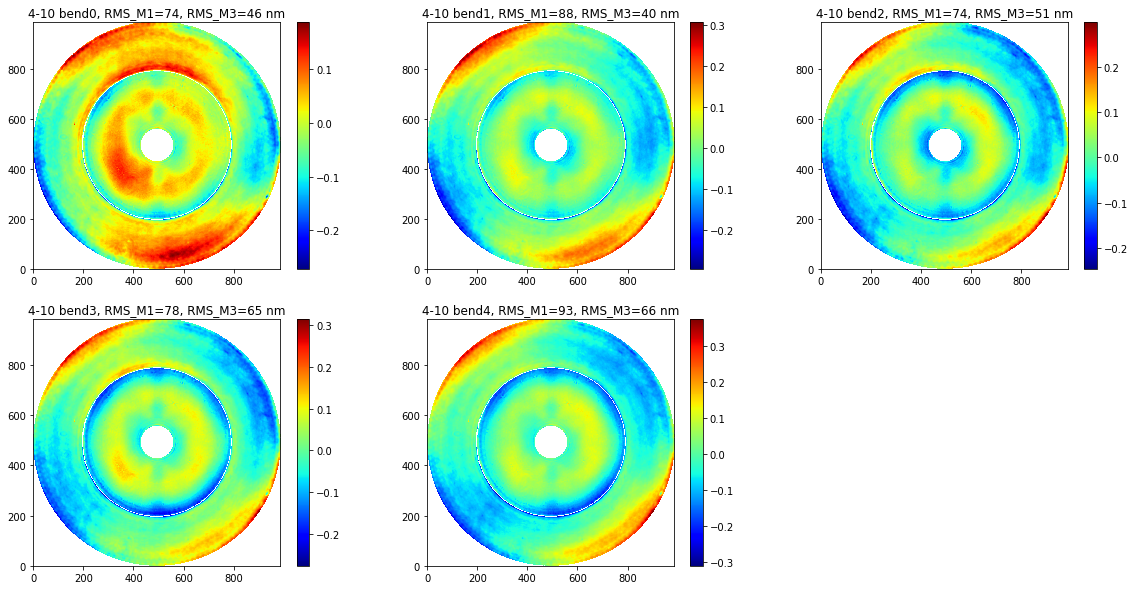
\includegraphics[width=150mm]{figures/reinstall.png}
  \end{tabular}
   \end{center}
   \caption
  { \label{fig:reinstall}
M1 and M3 surface maps before and after
removing and reinstalling the four actuators.
 }
\end{figure}


The RMS values of these difference maps are somewhat larger than the
20 nm measurement accuracy, but not much larger.
On the other hand, these difference maps seem to have structures that
are not consistent with being completely random.
We believe that this is due to technicians thermally disturbing the
environment inside the cell while removing and installing the actuators.

 \begin{figure}[bthp]
   \begin{center}
   \begin{tabular}{c}
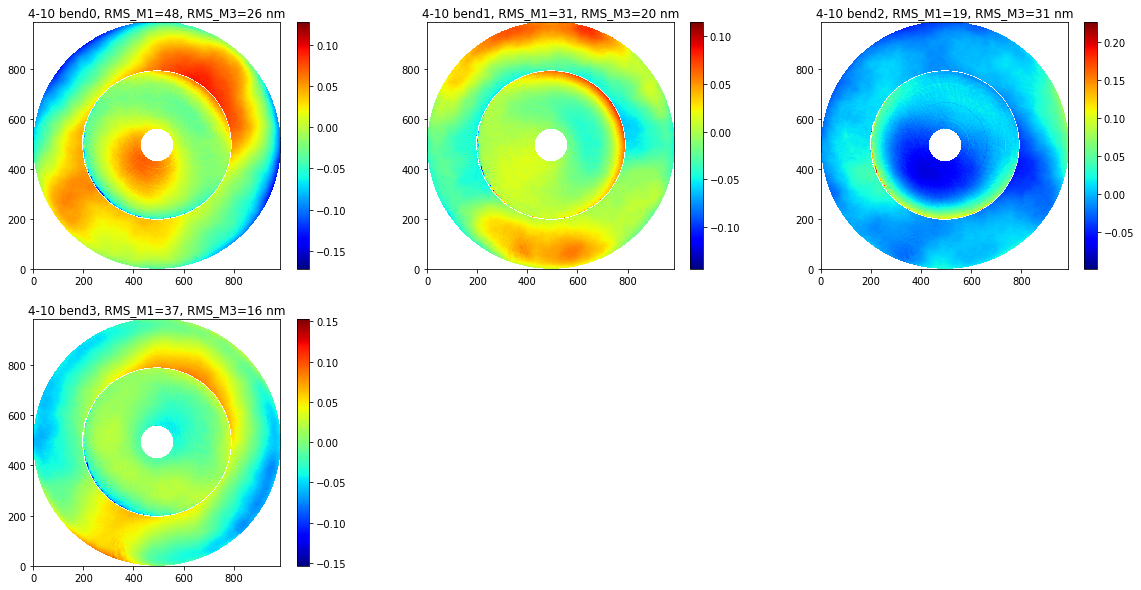
\includegraphics[width=150mm]{figures/reinstallDiff.png}
  \end{tabular}
   \end{center}
   \caption
  { \label{fig:reinstallDiff}
M1 and M3 surface difference maps between before and after reinstalling each actuator.
 }
\end{figure}

\section{Bending modes}

One of the major objectives of the Mirror Lab testing was to calibrate
the FEA-derived bending modes.

In this section, we first explain how we calculated the FEA bending
modes.
The actual bending mode measurements took place on 1/16, 1/17, and
2/11 for the Mirror Lab bending modes, and 2/13, 2/18, 2/19 for the
LSST bending modes.
The corresponding Jupyter Notebooks are
\bitm
\item \url{https://github.com/bxin/M1M3_ML/blob/master/190116.ipynb}
\item \url{https://github.com/bxin/M1M3_ML/blob/master/190117.ipynb}
\item \url{https://github.com/bxin/M1M3_ML/blob/master/190211.ipynb}
\item \url{https://github.com/bxin/M1M3_ML/blob/master/190213.ipynb}
\item \url{https://github.com/bxin/M1M3_ML/blob/master/190218.ipynb}
\item \url{https://github.com/bxin/M1M3_ML/blob/master/190219.ipynb}
\eitm

\subsection{FEA bending modes}
\label{sec:feaBM}
FEA bending modes calculation procedure is given in document-15312~\cite{m1m3bmcalc}.
Calculating the FEA bending modes is actually a non-trivial process.
It is important to make sure we get the most accurate results from the
FE model, because that is what we start with during the testing. 

As
a quick summary, it involves the following steps.
\bnum
\item Deriving the unit-load force vectors. Each unit-load force
  vector has one actuator that pushes with a 1000 N force, while all
  other actuators work together to offset the net $z$-force and the
  $x$ and $y$ moments. In solving for 155 forces under 3 constraints,
  we assume the 155 forces have a 2D linear distribution, therefore
  only 3 coeffients are needed to determine all 155 forces. These 156
  vectors, each has 156 elements, gives a matrix $C$, which is 156
  $\times$ 156.

  \item Applying the unit-load force vectors to the FEA model of the
    mirror, and outputing the resulting surface shapes. For our FEA
    model we have 5256 surface nodes, therefore each surface shape is
    a 5256 $\times$ 1 vector, and we have 156 of these vectors.
    These 156 vectors, each 5256 elements long, gives a matrix $D$,
    which is 5256 $\times$ 156.

    \item Calculcating mirror influence matrix $G$. Because $D = GC$,
      so we have $G = DC^{-1}$.

    \item Performing a singlar-value-decomposition (SVD) analysis of G, the output of which being all the
      bending modes and their corresponding force vectors. Since
      $G = U\Sigma V^T$, and $U$ and $V$ are unitary matrices, and we want
      to have bending modes with fixed surface RMS, e.g., RMS = 1
      $\mu$m, we scale $V$ to absorb $\Sigma$. Let $V^\prime$ be the
      bending mode force vectors, we can decompose any surface into
      $U\alpha$ and the corresponding force vector into $V^\prime \alpha$.
      \beq
      U\alpha = (U \Sigma V^T) V^\prime \alpha
      \eeq
      Therefore
      \beq
      V^\prime = V \Sigma^{-1} 
      \eeq
\enum

There are a few subtle decisions to make, once we start to think about
the details.
\bnum
\item 156 forces versus 256 forces. In principle, the above
  procedure can be applied to all 256 actuators, treating each
  cylinder, or equivalently, $F_y$ and $F_z$, as an independent actuator. Mathematically, this should
  give better results, because the lateral actuators can influence the
  mirror surface in $z$ as well. But, in reality, these two different methods make very
  little difference in results, and it is much cleaner to only use the $z$ forces
  to control mirror shape, $y$ forces to offload gravity when we point
  off-zenith, and $x$ forces for slewing and countering dynamics.

  \item Subtraction of piston-tip-tilt (PTT) components from the
    unit-load surface shapes. In principle these should not be
    subtracted, because FE analysis verifies that even when the hard
    points are constrained, the surface shape can still have PTT, as
    the mirror is not a rigid body. So PTT will be part of what we put
    on the mirror surface when we command those bending mode
    forces. But, in reality, the amount of adjustments these PTT
    components requires from the hexapods is less than the hexapod
    motion resolution. Also note that we subtract PTT
    separately from M1 and M3 unit-load shapes, because the two
    interferometers are independent during the testing.

  \item Surface sag, surface normal, versus $z$-displacements.
    For the purpose of testing the bending modes, we always use
    surface normal, because of the way interferometers work. The calibrated bending modes will also be in
    surface normal. But it is noted that when these bending modes are
    implemented in raytrace programs, they need to be projected to be
    surface sag, if that is how the distorted surfaces are
    defined. See Document-16390~\cite{m1m3sag} for the difference between the three.
\enum

We note that the Mirror Lab and LSST have maintained seperate FE
models of the M1M3 mirror. We also calculated the bending modes
separately. Before the testing started, we confirmed with each other
we have been following the same calculation procedure the best we know
it. However, due to differences in the FE models,
and the sensitivity of the bending modes calculation to numerical effects,
the two sets of
bending modes are a bit different.

For the bending mode measurements, which we will
talk about next, we started with the Mirror Lab bending modes. 
However, as time went on, it appeared that the LSST bending modes are more effective when used for
surface optimization.
In this document, we will mostly focus on the measured LSST bending modes.

The bending modes derived by the LSST team from the LSST FE model is
shown in Figure~\ref{fig:feaBM}. Here we show the first 30 modes.
The Active Optics System (AOS) baseline currently uses 20
modes. Considering numerical effects in the process of deriving FEA
bending modes, the ordering of the modes could be a bit uncertain. At
the beginning of the testing campaigns, the intention was to measure the
first 22 bending modes. Later on during the surface optimization
process, it was determined that bending mode No. 27 was needed for
optimizing the mirror surface.
We therefore measured modes 1-27.
This will be discussed in detail later in Section~\ref{sec:finalBM}. 

 \begin{figure}[bthp]
   \begin{center}
   \begin{tabular}{c}
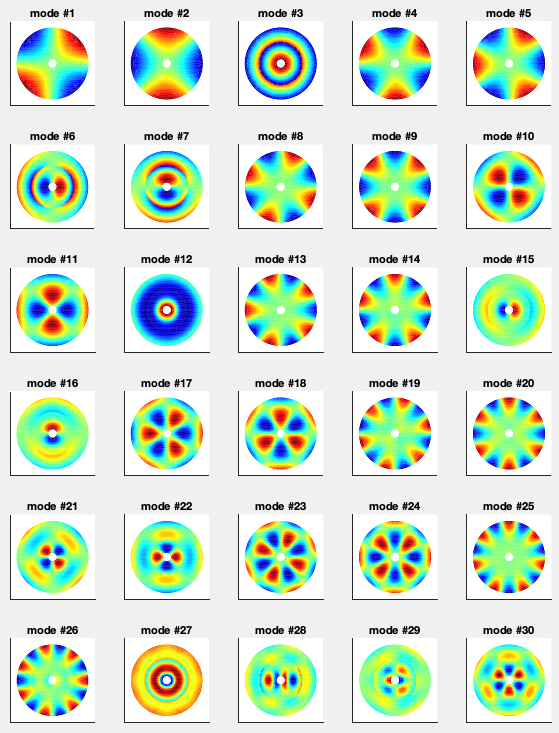
\includegraphics[width=140mm]{figures/feaBM.png}
  \end{tabular}
   \end{center}
   \caption
  { \label{fig:feaBM}
Bending modes determined by the LSST team using the LSST FE model.
 }
\end{figure}

\subsection{Measured bending modes}

To measure a bending mode $B_i$, we take the FEA-predicted forces for the
mode $F_i$, apply them, then measure the change in the surface shape.
The base force set $F_0$, just like the one used in the repeatability
test, is from one of the preliminary surface optimizations. It is a
differential measurement, so details in $F_0$ doesn't matter much.

To further remove possible thermal drifts during the process, and to
lower the error on the measurements, we always followed the following
procedure:
\bnum
\item apply $F_0+F_i$, measure mirror surface to get $S_{+1}$;
  \item apply $F_0-F_i$, measure mirror surface twice to get $S_{-1}$ and
    $S_{-2}$;
    \item apply $F_0+F_i$, measure mirror surface to get $S_{+2}$;
      \enum
      We call this a $+--+$ measurement.
      In reality, we want these forces to produce surfaces with RMS of
      roughly 500 nm, so that the surface measurements would be of
      good accuracy. So most of the time the actual $F_i$ is a scaled
      version of the FEA determined force set $F_i^{FEA}$. The actual
      RMS values for each bending mode, for M1 and M3 separately, are
      listed in Table 5 of the Mirror Lab analysis document~\cite{m1m3UAreport},
      therefore not repeated here.

Because measuring M1 surface requires stowing the M3 bridge, instead
of finishing both M1 and M3 surface measurements for a bending mode
then moving onto the next bending mode, we always did the above for many
M1 modes before moving onto the same set of M3 modes.

      The measured bending mode (for M1 or M3) is
      \beq
      B_i = \frac{S_{+1} + S_{+2} - S_{-1} - S_{-2}}{2} \times
      \frac{RMS(F_i^{FEA})}{RMS(F_i)}.
      \eeq

 As examples, Figure~\ref{fig:m1pmmp} shows the $+--+$ measurements
 for M1 bending modes No. 17, 18, and 20.
 The resulting measured bending modes, for both M1 and M3, are shown
 in Figure~\ref{fig:measuredBM}.
 We do not want to fill this document with plots. If a reader is
 interested in looking at other modes, the Python notebooks in the
 GitHub rep would be a good place to look. All the data files are
 included in the data package delievered by the Mirror Lab. The path
 to the files can be found in the Python notebooks.
      
 \begin{figure}[bthp]
   \begin{center}
     \begin{tabular}{c}
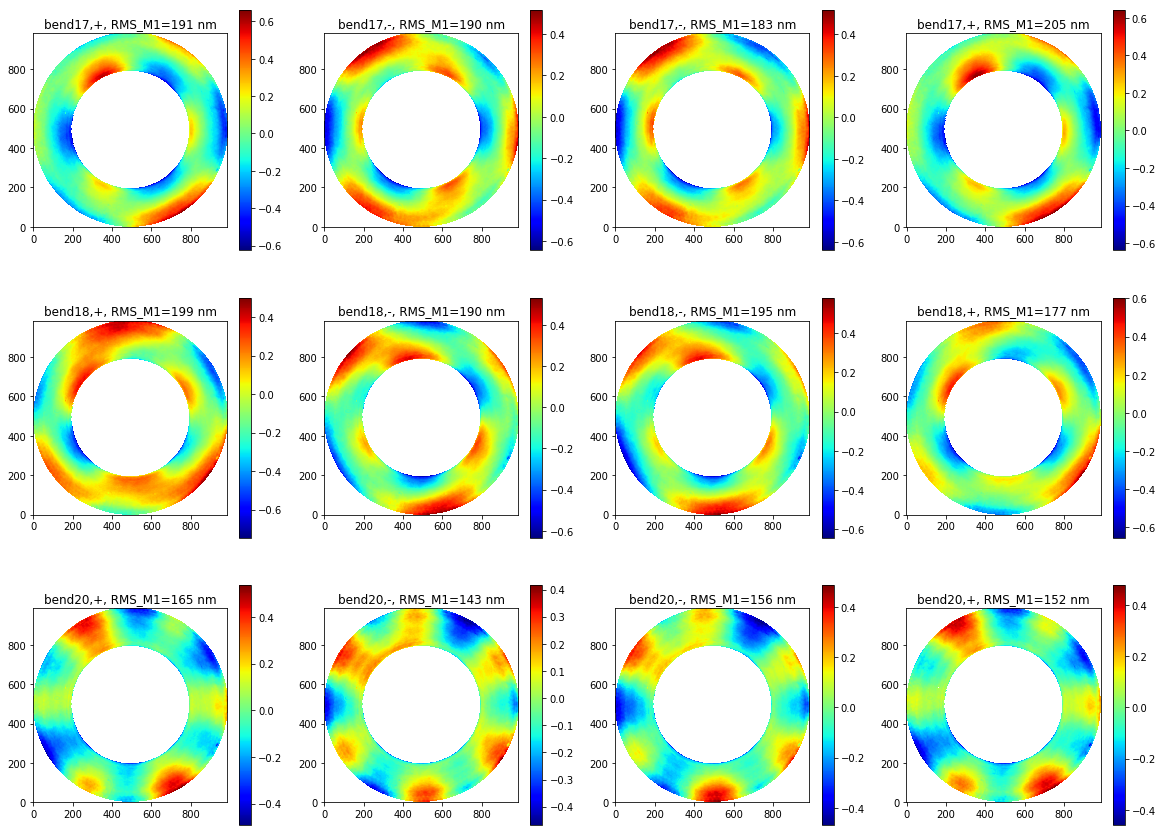
\includegraphics[width=150mm]{figures/m1pmmp.png}      
  \end{tabular}
   \end{center}
   \caption
   { \label{fig:m1pmmp}
     M1 $+--+$ measurements
 for the LSST bending modes No. 17, 18, and 20.
 }
\end{figure}

 \begin{figure}[bthp]
   \begin{center}
     \begin{tabular}{c}
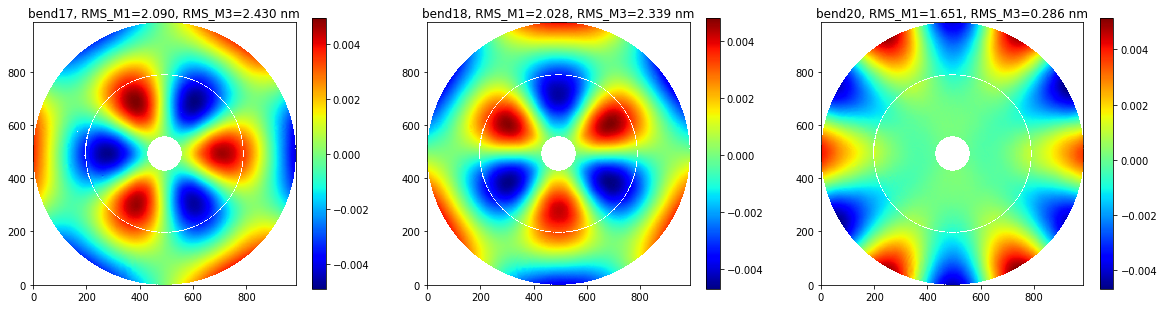
\includegraphics[width=150mm]{figures/measuredBM.png}
  \end{tabular}
   \end{center}
   \caption
  { \label{fig:measuredBM}
Measured LSST bending modes No. 17, 18, and 20.
 }
\end{figure}

\subsection{Bending Modes Scaling Factors and Cross-Talks}
\label{sec:finalBM}

As can be seen from Figure~\ref{fig:measuredBM} and many other
measured bending modes, the measured modes shapes are so much like the
FEA bending modes. This gives us confidence that the difference
between the measured modes and the FEA modes is mostly a scaling
factor, and it is very close to 1.

We next try to determine the scaling factors, and any cross-talk
between the bending modes. To do this, we take each measured bending
mode $B_i$, and make a least-square fit using 27 FEA bending modes. The fit
gives us 27 coefficients, among which $c_i$ is close to 1, while all
the other 26 coefficients should be close to 0.
We follow the Mirror Lab analysis, and define the residual of the fit as
\beq
R = (B_i - c_i B_i^{FEA}) \times
      \frac{RMS(F_i)}{RMS(F_i^{FEA})}..
\eeq
The residual maps for bending modes No. 17, 18, and 20 are given in Figure~\ref{fig:residualBM}.

 \begin{figure}[bthp]
   \begin{center}
     \begin{tabular}{c}
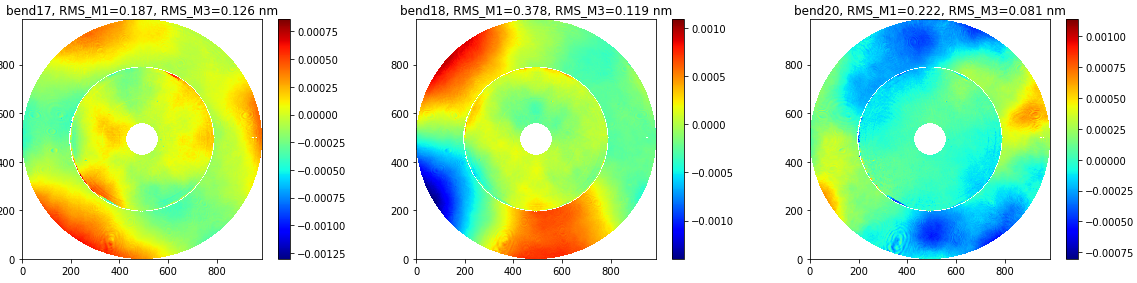
\includegraphics[width=150mm]{figures/residualBM.png}
  \end{tabular}
   \end{center}
   \caption
  { \label{fig:residualBM}
Bending mode residual maps for LSST mode No. 17, 18, and 20.
 }
\end{figure}

The $c_i$'s from the fits, which are the scaling factors that need to
be multiplied with the FEA bending modes to make them better match reality,
are shown in Figure~\ref{fig:scalingF}.
These scaling factors, for both the LSST bending modes and the Mirror
Lab bending modes, are shown together.
As another test of the repeatability, four of the the Mirror Lab modes
were repeated. The repeated bending modes measurements gave very
consistent results on the scaling factors as the original
measurements, as can be seen from Figure~\ref{fig:scalingF}.

 \begin{figure}[bthp]
   \begin{center}
     \begin{tabular}{c}
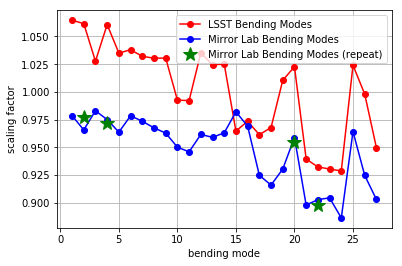
\includegraphics[width=100mm]{figures/scalingF.png}
  \end{tabular}
   \end{center}
   \caption
  { \label{fig:scalingF}
Scaling factors that need to be applied to the FEA bending modes.
 }
\end{figure}


A scaling factor less than 1 means FEA model is more flexible
than the real mirror. This is true for all the Mirror Lab bending modes.
For LSST, the lower order modes ($<$15) are generally stiffer than the real
mirror. We note that the Mirror Lab analysis report~\cite{m1m3UAreport} made fits
to LSST bending mode measurements using Mirror Lab FEA modes. We
believe that that is not meaningful, and could lead to confusion. Due
to numerical effect in FE modelling and derivation of the bending
modes, the two sets of FEA bending modes look similar but have visible
difference, especially in the orientations of the modes. Therefore, the
bending mode measurements made using LSST bending mode forces should be fit using
LSST bending modes. Otherwise the fits lead to very large cross-talk
terms, especially between modes that form pairs, for example, the two astigmatism modes, two coma modes, and so on.

Figure~\ref{fig:crossTalk} shows the cross-talk matrix of the bending
modes, where the $j$th column, $i$th row, shows when the force set for
the $j$th bending mode was applied, how much of bending mode $i$ was produced.
Most of the low order modes ($<$15) are very clean - they are free of
contaminations from higher order modes.
For higher order modes ($>=15$), the contamination is up to $\sim 15\%$.

 \begin{figure}[bthp]
   \begin{center}
     \begin{tabular}{c}
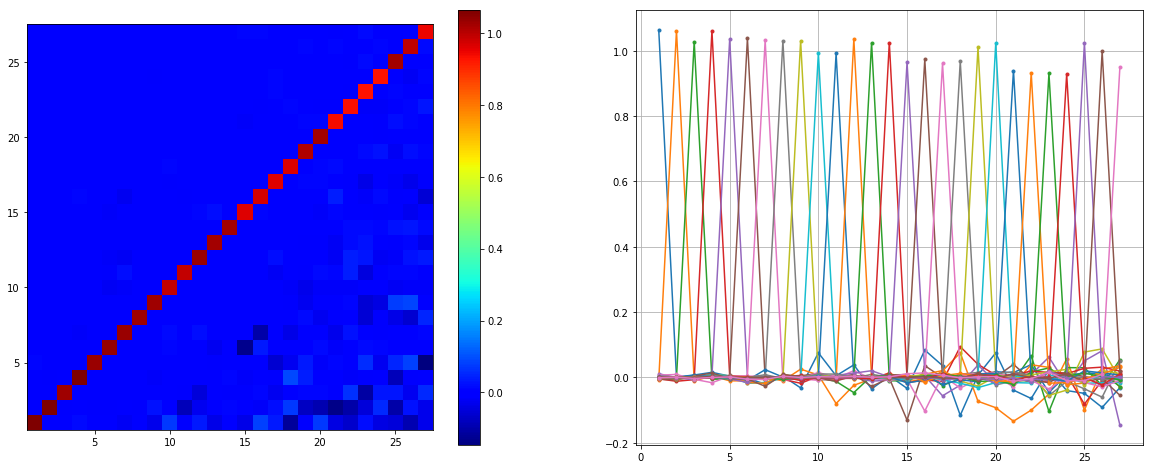
\includegraphics[width=150mm]{figures/crossTalk.png}
  \end{tabular}
   \end{center}
   \caption
  { \label{fig:crossTalk}
Cross talk matrix between the measured LSST bending modes (left), and the
projection onto the column index (right).
 }
\end{figure}

Because the FEA bending mode are free of measurement noise, and are
much smoother than the measured modes, we 
choose to apply the scaling factors on the FEA bending modes, and use
the scaled modes as the baseline bending modes to go onsky.

\subsection{Final Bending Modes}

What the cross talk matrix means, is, mathematically,
\beq
\left[ \begin{array}{c} m1  \\ m2 \\ \vdots \\ m27 \end{array} \right]
= X^T
\left[ \begin{array}{c} U1  \\ U2 \\ \vdots \\ U27 \end{array} \right]
= X^T G
\left[ \begin{array}{c} V1  \\ V2 \\ \vdots \\ V27 \end{array} \right].
\eeq

$X^T$ is the transpose of the cross-talk matrix $X$.
m1, m2, ..., m27 are measured mode shapes. U1, U2, ..., U27 are FEA mode shapes. These are all matrix blocks, each is a nNode x 1 vector. nNode is the number of surface nodes. 
V1, V2, ..., V27 are FEA force sets. These are matrix blocks too, each being a 156 x 1 vector. G is the FEA influence matrix, which is nNode $\times$ 156.

Noticing that when we applied V1, V2, ..., V27 forces in the Mirror Lab, we measured m1, m2, ..., m27. $X^T G$ actually gives us the real influence matrix ($g$).
\beq
g = X^T G
\eeq

We want to keep our mode shapes orthonormal, so we keep
using U1, U2, ..., U27 as our bending mode shapes,
and scale the forces.
Now, what we want to derive is the force sets that would give us U1, U2, ..., U27 in the real world.

\beq
\left[ \begin{array}{c} f1  \\ f2 \\ \vdots \\ f27 \end{array} \right]
= g^{-1}
\left[ \begin{array}{c} U1  \\ U2 \\ \vdots \\ U27 \end{array} \right]
= g^{-1} G
\left[ \begin{array}{c} V1  \\ V2 \\ \vdots \\ V27 \end{array} \right]
= (X^T G)^{-1} G
\left[ \begin{array}{c} V1  \\ V2 \\ \vdots \\ V27 \end{array} \right]
\eeq

So, to know f1, f2, ..., f27, all we need to know is the matrix $m$,
\beq
m = (X^T G)^{-1} G = (X^T)^{-1} 
\eeq

Note that $G$ is a matrix that applies to the matrix blocks
above. Each element of the 27 $\times$ 27 matrix $X^T$ is mutliplied with
$G$. Therefore $G$ is commutable with $X$.

Ideally, we want to make use of the full cross-talk matrix, i.e.,
multiply the $m$ matrix with the $V$ vectors, to get the final $f$
force vectors which would produce the $U$ bending modes.
However, attempting to do so resulted in wierd-looking force
distributions for the bending modes, as shown in the notebook
\url{https://github.com/bxin/M1M3_ML/blob/master/finalBendingModes.ipynb}.

We therefore decided to set all the off-diagonal elements of $m$ to
zero. This is basically saying that we will ignore the measured
cross-talks between the bending modes, and assume those are due to
measurement noise and environmental drifts.
This is equivalent to using a simple measured scaling factor to scale
the forces for each bending mode.

The final bending mode forces after the scaling is found at
\url{https://github.com/bxin/M1M3_ML/blob/master/data/M1M3_1um_156_force.txt}.
Each row is for an actuator. There are 156 rows in total.
The first column is the actuator ID. The 2nd and 3rd columns are the x
and y coordinates of the actuators. The rest of the columns are forces
for individual bending modes in Newton.
The bending mode shapes are at
\url{https://github.com/bxin/M1M3_ML/blob/master/data/M1M3_1um_156_grid.txt}
Each row is for a surface node. There are 5256 rows in total. The
first column is the node ID. The 2nd and 3rd columns are the x and y
coordinates in meter for that node. The rest of the columns are for
individual bending modes. Note that these are surface normal
displacements in meter, which need to be projected to surface sag if
used in raytrace programs.

\section{Single actuator influence functions}

To help better understand the difference between the mirror FE model
and the real mirror, we also measured 50 single actuator influence
functions. There is nothing special about the number 50. After some
number of single actuator influence function measurements, this
became a low-priority task. We basically filled the time when other
tasks were not ready to be executed.
In the end, 50 was what we could get out of the time we had in the
Mirror Lab.

The way we determined which influence functions to measure was to pick
a set of actuators that represent a variety of types, including number of
cylinders, their orientation, and load spreader type, and radial and
athimuth location in the mirror cell.
The LSST team made a list of 60 actuator ID numbers, ranked them by
priority from high to low, and gave those to the mirror lab crew.
The distribution of these 50 actuators are shown in
Figure~\ref{fig:IFdist} (left), where the same coordinate system as in
Figure~\ref{fig:cs} has been used. We focused on the 4th quadrant,
where the actuator ID numbers are in the 100's range.
Some actuators in the other quadrants were added to the list, mostly
to check symmetry.

 \begin{figure}[bthp]
   \begin{center}
     \begin{tabular}{c}
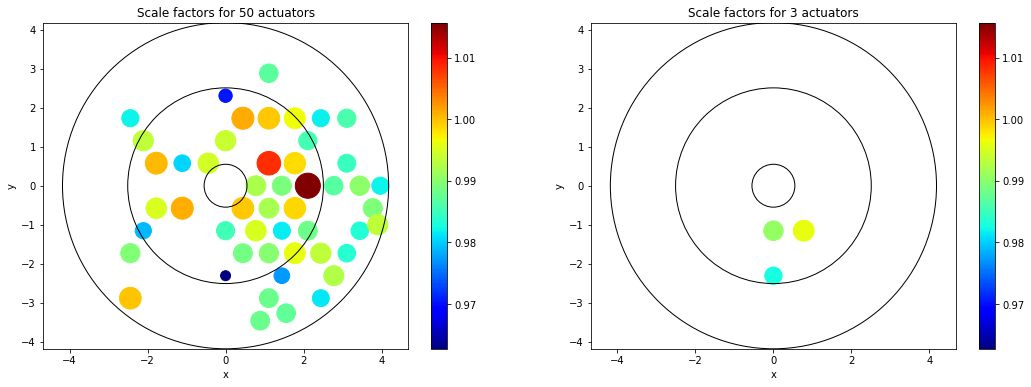
\includegraphics[width=150mm]{figures/IFdist.png}
  \end{tabular}
   \end{center}
   \caption
   { \label{fig:IFdist}
     Measured single actuator influence function scaling factors
     versus their $x$ and $y$ coordinates. These are in the coordinate
     system as defined in Figure~\ref{fig:cs}.
     All 50 actuators measured are shown in the left plot, and the
     right plot shows the 3 actuators that were repeated on a
     different day.
Note that the color scales on the two plots are the same. The size of
the circles are relative to other circles on the same plot, therefore
not comparable between the two plots.
 }
\end{figure}

The single actuator influence function measurements were done in a
very similar way as the bending modes.
For each actuator, we take the unit-load forces, as described in
Section~\ref{sec:feaBM}, and add a
scaling factor so that the FEA-predicted surface would roughly have a
RMS of 500 nm.
The scaled force for the single actuators, which are also the largest
forces among their own unit-load force sets, are listed in Tables 3
and 6 of the Mirror Lab analysis report~\cite{m1m3UAreport}, therefore not repeated here.
Just like for the bending modes, we did $+--+$ measurements;
and we did 
this for M1 and M3 separately,
i.e., M1 surface measurements for a series of scaled unit-load forces,
followed by M3 surface measurements for a series of scaled unit-load
forces.
For the same influence function,
the scaling factors were allowed to differ between M1 and M3, to
achieve surface RMS of roughly 500 nm in each case.

The fits to the measured single actuator influence functions using
their FEA predictions also
follow a similar approach as the fits to the bending modes.
The major difference is that instead of fitting to 27 bending modes,
here the least-square fits are only done using one FEA influence
function at a time.
Figure~\ref{fig:IFeg} shows two examples of such fits, for actuators
102 and 138, representing actuators under M3 and M1, respectively.
The first column shows the measured influence functions.
The second column shows the FEA predicted influence functions.
The third column shows the fit result, i.e., the fitted scale factor
times the second column.
The fourth column shows the residual of the fits, scaled to 1N of
RMS force on the selected actuator.
The circles indicate the locations of the selected actuator. 
Good agreement between the measured influence functions and the FE
model was seen, in terms of both the magnitude and overall shape.
The scale factor for actuator 102 was determined to be 0.989, and for
actuator 138 it was 0.988.

 \begin{figure}[bthp]
   \begin{center}
     \begin{tabular}{c}
       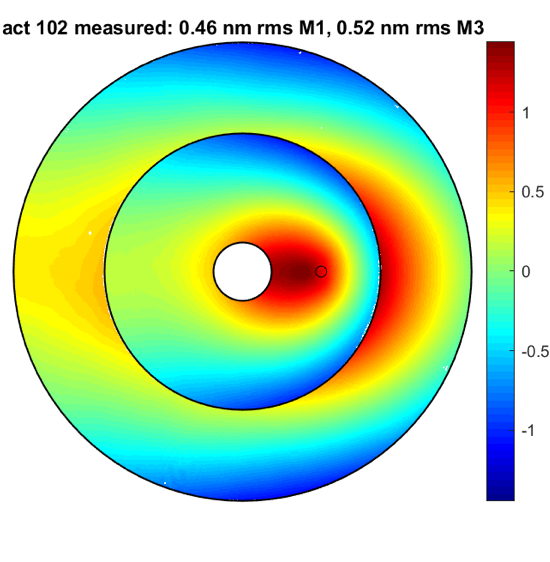
\includegraphics[width=40mm]{figures/if102m.png}
       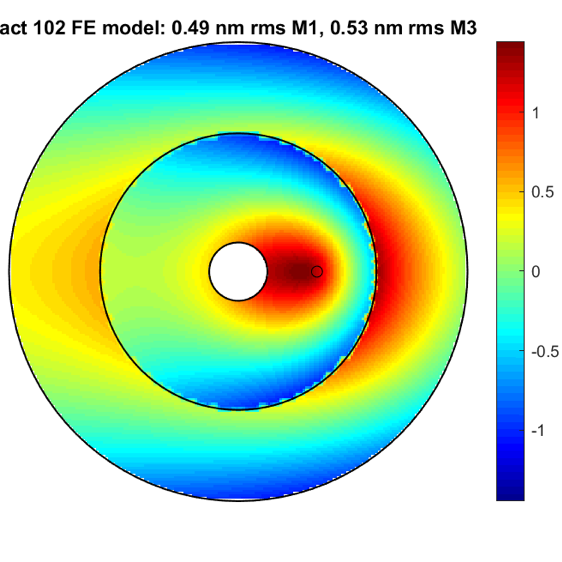
\includegraphics[width=41mm]{figures/if102f.png}
       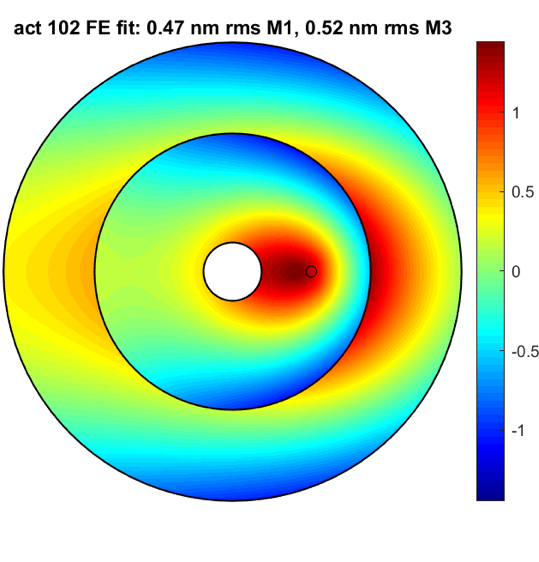
\includegraphics[width=40mm]{figures/if102fit.png}
       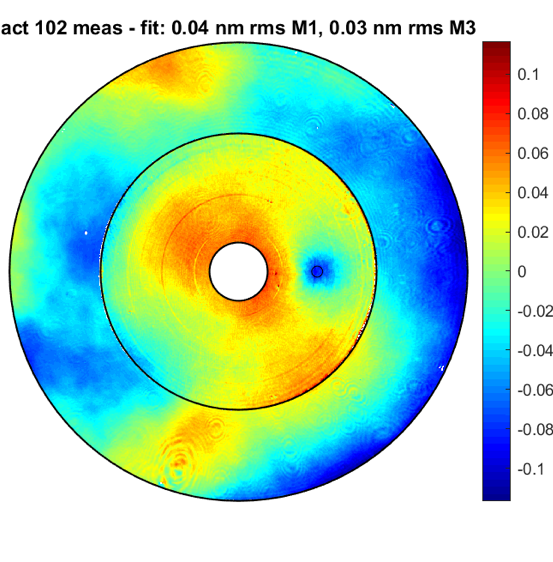
\includegraphics[width=41mm]{figures/if102r.png} \\
       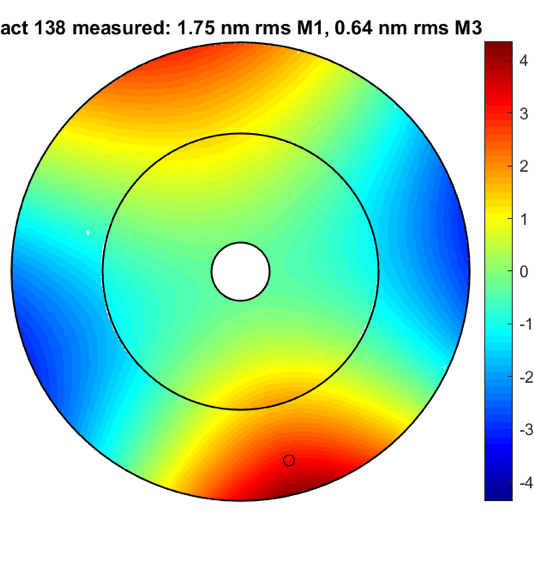
\includegraphics[width=40mm]{figures/if138m.png}
       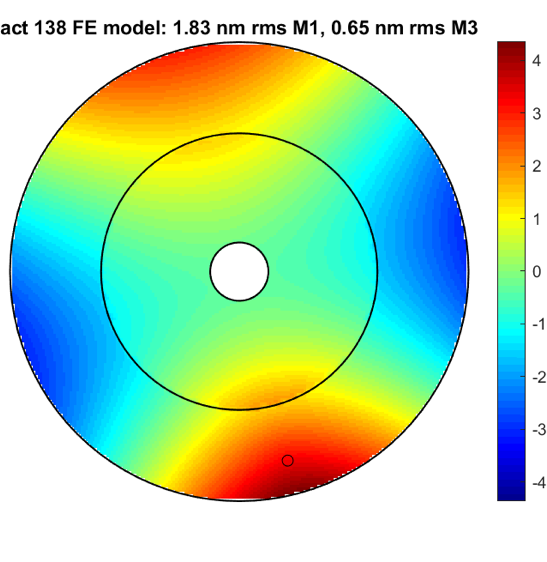
\includegraphics[width=41mm]{figures/if138f.png}
       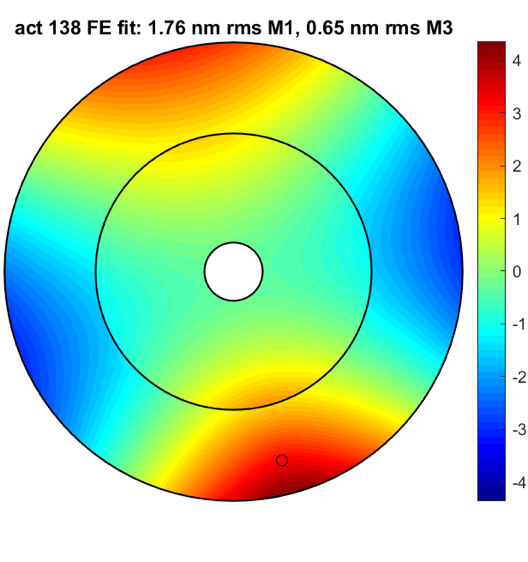
\includegraphics[width=40mm]{figures/if138fit.png}
       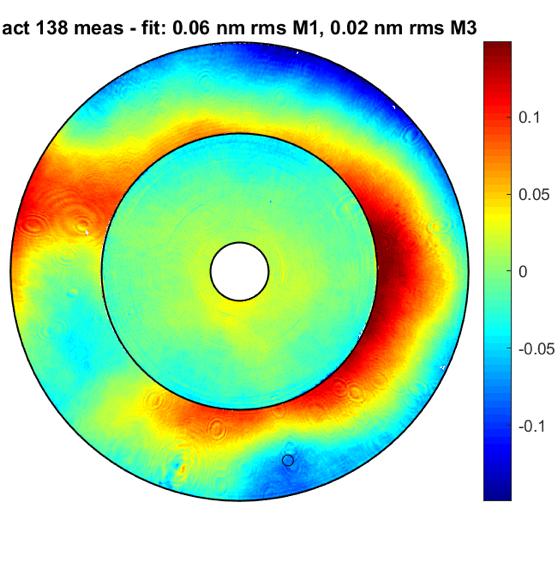
\includegraphics[width=41mm]{figures/if138r.png} 
  \end{tabular}
   \end{center}
   \caption
   { \label{fig:IFeg}
     Measured single actuator influence functions (1st column), the
     corresponding FEA predicted influence functions (2nd column), the
     fitted surfaces to the FEA influence functions (3rd column), and
     the residual of the fit (4th column) for two example actuators -
     102 (top row) and 138 (bottom row).
 }
\end{figure}

It was observed that for all actuators under M3, the residual maps
have localized spots that are negative (blue). This implies that the real
mirror is stiffer against shear than the FE model.
For M1, the residual maps generally show more blue than red on or
around the selected actuator positions. But the locality is much less pronounced.

Note that the single actuator measurements were done only
using the Mirror Lab FEA influence functions.
Since we do not use the results presented in this section in any 
quantitative calibration of the FE model or the final bending modes,
we did not make comparions between the Mirror Lab FEA influence
functions and those derived from the LSST FE model, nor the force
vectors for those single actuator influence functions between LSST and
the Mirror Lab.
We did not repeat the influence function measurements (if the
unit-load forces
are different) for LSST influence functions.

The values of the scale factors to be applied to the FEA single
actuator influence functions are shown in Figure~\ref{fig:IFdist}
(left).
The scale factors to be applied to the FE influence functions range
between 0.96 $-$ 1.02.
To check the repeatability of these measurements, we redid these for
three actuators on a different day. The resullts on are shown in
Figure~\ref{fig:IFdist} (right).

All results in this section show consistent agreement between the FEA single actuator
influence functions and those measured for the real mirror.
The detailed analysis in Jupyter Notebook format is documented in
\bitm
\item \url{https://github.com/bxin/M1M3_ML/blob/master/190118.ipynb}
\item \url{https://github.com/bxin/M1M3_ML/blob/master/190122.ipynb}
\item \url{https://github.com/bxin/M1M3_ML/blob/master/190214.ipynb}
\item \url{https://github.com/bxin/M1M3_ML/blob/master/190218.ipynb}
  \eitm

\section{Surface optimization}

The surface optimization was what took the most time in the Mirror
Lab. But at the end, we achieved superb surfaces on both M1 and M3. We
will present the results later in this Section~\ref{sec:optS}.
Looking back at the whole process, from turning on the system at the
beginning of the test campaigns to eventually
achieving the final optimized surfaces, here is a list of key things
that we had to do to get there.
\bnum
\item M1M3 global optimization
\item use of LSST bending modes
  \item correct calculation of the initial forces 
  \item understanding the divits above the quads
    \item undertanding the absolute offset in actuator forces
  \item use of bending modes up to 27 
\enum

No 1 and 2 above are the eaisest to explain. We describe them here in
a bit more detail, then go through 3 - 6 in the sub-sections.
The analysis is spread into many notebooks. We will refer to those
where relevant.

Initially we only
iterated the optimization process using M1 surface measurements, but
only to find that M3 drifted a lot during that process.
So we decided to do the M1-M3-M1 measurements, then fit the M1M3
combined surface to the M1M3 combined bending mode shapes.
Note that when the mirror was polished back in circa 2014, the Mirror
Lab was able to polish M1 first, fit M1 surface to low order bending
modes, then use those bending modes as the target shape during M3
polishing. That was because the data processing at that time included
thermal corrections. So the mirror shape measured then were always in
reference to the shape in a pre-defined thermal condition.

At the beginning of the surface optimization process, we used the
Mirror Lab bending modes. At some point we decided to give the LSST
bending modes a try. The LSST bending modes appeared to be
more effective while used in these optimizations. They resulted in
somewhat better surfaces, and the convergence toward better surfaces
were noticeably faster.
We do not think the LSST bending modes are inherently superior in any  
way.  
As we mentioned earilier, we believe the bending mode derivations are
identical between LSST and the Mirror Lab. So the difference in these
two sets of bending modes most likely reside in the two different FE
models that were used. It may be that the LSST FE model went through
may refinements and have better representation of the material properties.

\subsection{Initial force calculation}
\label{sec:initF}

The plan was to start the surface optimization with the support forces
from the 2014 acceptance testing. Then, hopefully the surface shape
change due to the different thermal environment can be taken care of
using 20 or so low order bending modes.
However, we shouldn't just use the support forces the way they were in
2014, because some of the mirror support hardware have changed between
then and now. The initial force calculation has to take that into
account.

This calculation may sound trivial - starting from the 2014 forces,
one simply removes the weights of the Mirror Lab hardware which had been removed
since then, and add the new LSST hardware weights.
Based on that, we put together a Notebook - \url{https://github.com/bxin/M1M3_ML/blob/master/sec3.2InitialForces.ipynb}.
However, this is not as simple as one might first think, mostly
because the Mirror Lab actuators were all SAAs, while most of the LSST
actuators are DAAs. With the secondary cylinders of the DAAs oriented at
45$^\circ$ relative to the primay, we have to command some non-zero
forces on the secondary cylinder, to keep the primary cylinder at
vertical position, just like when the DAAs are free-standing.
The actual mathematical derivation of the initial force set is rather tedious,
therefore not documented here. Instead, they are found in a separate
document, 
Document-32192~\cite{m1m3initF}.
That document also gives analytical results for off-zenith
pointings. These will need to become part of the M1M3 look-up-table (LUT).
The numerical calculations are found here - \url{https://github.com/bxin/M1M3_ML/blob/master/sec4.3InitialForces.ipynb}.


\subsection{Divits above the quads}
\label{sec:divits}

Very early on in the test campaigns, even where we used M1 only for
the surface optimizaiton, we observed 4 low spots on the M3
surface, roughly right on top of the four actuators whose load
spreader has 4 pucks. We call those four actuators the quads.
Figure~\ref{fig:divits} shows the optimized M1 and M3 surface together from
an optimization on 2/12. This particular optimization was done using
the Mirror Lab bending modes, and was an M1M3 global
optimization. Four dark blue spots can be clearly seen on top of the quads.
See \url{https://github.com/bxin/M1M3_ML/blob/master/190212.ipynb} for
more details.
  
 \begin{figure}[bthp]
   \begin{center}
     \begin{tabular}{c}
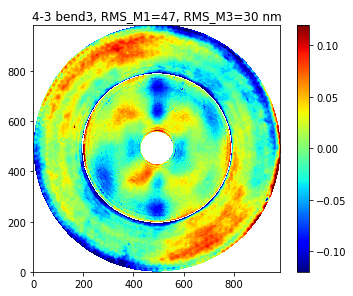
\includegraphics[width=80mm]{figures/divits_190212.png}
  \end{tabular}
   \end{center}
   \caption
   { \label{fig:divits}
     Measured M1M3 surface on 2/12, where no additional forces were
     added to the quads, and optimization was done using 27 Mirror
     Lab bending modes.
 }
\end{figure}


Our first reaction was that there is some kind of force offset that
was not properly accounted for. And, irregardly of the reason, just 
bumpimg up the forces on the quads should fix it.
It turned out that simply increasing the forces on the four quads
didn't work out very well.
Just looking at the depth of these low spots, and using the single
actuator influence functions, we could estimate how much forces would be
needed to bring these spots up.
Figure~\ref{fig:quadsUp} shows the M1M3 surface we got by adding 350N to the outer
     quads, and 300N to the inner quads, then optimizing using 27 Mirror Lab
     bending modes.
     The divits seem to be less visible, but the overall RMS on M1 and
     on M3 did not get better, as shown in the titles of these plots.
   This is also found in \url{https://github.com/bxin/M1M3_ML/blob/master/190212.ipynb}.
     
 \begin{figure}[bthp]
   \begin{center}
     \begin{tabular}{c}
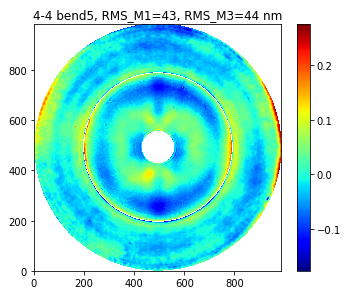
\includegraphics[width=80mm]{figures/quadsUp.png}
  \end{tabular}
   \end{center}
   \caption
   { \label{fig:quadsUp}
     Measured M1M3 surface on 2/12, where we added 350N to the outer
     quads, and 300N to the inner quads, and optimization was done using 27 Mirror
     Lab bending modes.
 }
\end{figure}

Another problem we ran into with simply increasing the forces on these
quads was that we kept triggering the safety limits of the M1M3
control software, specifically, the near neighbor check.
In order to avoid the situation where one actuator is acting
dramatically differently from its N near neighbors, which could
impose a danger to glass safety, we require the
force on any single actuator to be within a certain range from the
average of its N neighbors. Most of the time we have N = 6.
\beq
F_i - \frac{\sum_{j=1}^{N} F_j}{N} <= c \frac{W_{M1M3}}{156}.
\eeq
$W_{M1M3} $ is the weight of the mirror. We have $W_{M1M3} \approx 167,000$ N. By default, we set $c$=1.
So this requires the above difference to be less than $\sim$1070N.
If the above condition is triggered then the mirror goes into a fault
state - the mirror will be lowered, and we have to start over by
raising the mirror.
In addition to the near neighbor check, there are also other safety
checks, including the moment check, weight check, Active Optics force
check, and a far neighbor check. The far neighbor check is very similar to near neighbor
check, with N = 12. It is aimed at protecting the mirror from large
global bending.


Of course, we thought hard on what could be causing these so
localized features. In other words, what could have changed between
mirror acceptance in 2014 and 2019, that lead to such difference in
the mirror surface shape.
With the analysis described in Section~\ref{sec:initF} and Ref~\cite{m1m3initF},
for a while, we believed we had accounted for everything
properly. Then we started questioning the absolute force calibration
of these actuators. The relative force calibration was done before the
individual actuators were installed, meaning that we are pretty
confident when we command an actuator to increase the force by
$dF$, the load cells show the increase is $dF+e$, where $e$ is fairly
small in this context, according to Section.~\ref{sec:ferror}, the actual
force increase is not far from $dF$ either.
But, could the absolute calibration be so much off, i.e., when we
think we are applying 1800 N force, it is actual only outputing 1500
N?
That sounds impossible, because all these DAAs are the same. We cannot
think of a reason that the DAAs installed under the quads are so much
off while other DAAs installed under the triples have offsets that are
close to zero. Still, since we had a few spare DAAs laying in the lab,
we conducted some measurements by letting these free-standing DAAs,
without any loads, to
stand vertically, and also lay on their sides. Then we measure the
load cell readings. The results are documented in Ref.~\cite{divitFEA}
where they are also compared to analytical calculations found in
Ref.~\cite{m1m3initF}. Good agreement was found.
This resulted in a future to-do item, which is to measure the absolute
force offset of all the load cells after all the actuators are detached from the
mirror back surface. The actuators will need to be detached for shipping to Chile anyway.

We also noticed that these localized features on the mirror surface,
are actually of higher spatial frequency than the actuators could
possibly correct. Figure~\ref{fig:quads153} shows the surface we get
if we take the surface measured, as shown in Figure~\ref{fig:divits},
fit to all 153 bending modes, then subtract off the result of the
fit. Note that we have 153 bending modes because the bending modes
have to satisfy 3 constraints: $z$ net force is zero, and $x$ and $y$
moments are zero. This is basically saying, Figure~\ref{fig:quads153}
shows the best surface we could possibly get by adjusting all the
actuators. The surface RMS values are small, but the pattern on the
surface is still visbble. So this is higher spatial frequency than the
actuators can create or compensate.
More details are found in \url{https://github.com/bxin/M1M3_ML/blob/master/190212.ipynb}.

 \begin{figure}[bthp]
   \begin{center}
     \begin{tabular}{c}
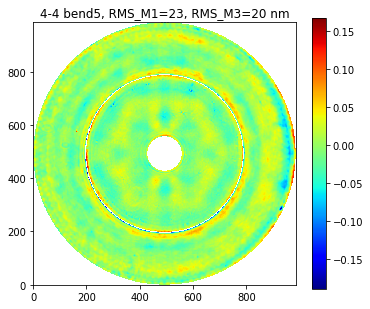
\includegraphics[width=80mm]{figures/quads153.png}
  \end{tabular}
   \end{center}
   \caption
   { \label{fig:quads153}
     FEA prediction of best M1M3 surface we could achieve by force optimization.
     This was obtained by taking the measured surface as shown in
     Figure~\ref{fig:divits}, make fit to, then remove all 153 bending modes.
 }
\end{figure}

Eventually, we figured out that it must be due to the following: there
has been a change in the way the quads are supported. Due to mirror
design, these quads require larger forces than other actuators to
support the mirror against gravity. That is why they are quads - with
4 pucks.
During mirror polishing, the Mirror Lab did not have strong enough
actuators to be used under these quads, so they used two actuators
under each quad. That is why, as mentioned in document-32192~\cite{m1m3initF}, the
Mirror Lab initial force set had 160 values, and they had 160
interface plates. The two actuators for each quad was on the two sides
of the load spreader. With the LSST mirror cell, those pairs of
actuators were replaced with single DAAs, which supports the 4-puck
load spreaders at the center. In the later case, the load spreaders
acted like bridges. With support forces around or larger than 1500 N,
lateral forces and moments are created, which push the contact points
on the mirror back surface outwards. As a result, low spots are
created on the front surface.

Optimizing the mirror surfaces with the FE model gave roughly same
forces as those as used to produce the surfaces shown in
Figure~\ref{fig:divits}.
To be specific, we subtracted the forces used to produce the surfaces shown in
Figure~\ref{fig:divits} from the FEA predicted optimized forces.
When we looked at the force difference map, we didn't observe any
large spikes around the quads.
This is because the shear forces and moments are not present in the finite
element model. The finite element model does model the pucks of the
load spreaders. But all it does is to evenly distribute the forces
applied by individual actuators onto the pucks, by treating the load
spreaders as perfectly rigid.

To check whether the lateral forces are the real cause here, Ed
Hileman modeled the individual load spreaders as flexible structures.
Shear forces were derived from the FE model, with typical large axial forces
exerted on the load spreaders. These shear forces are then added to the
mirror FE model together with all the other actuator forces. The
resulting M1 and M3 surfaces were shown to be very close to the actual
measured surface with the 4 divits.
For readers' convenience, the modeled surfaces with lateral forces are
also included here, in Figure~\ref{fig:divitsFEA}.


 \begin{figure}[bthp]
   \begin{center}
     \begin{tabular}{c}
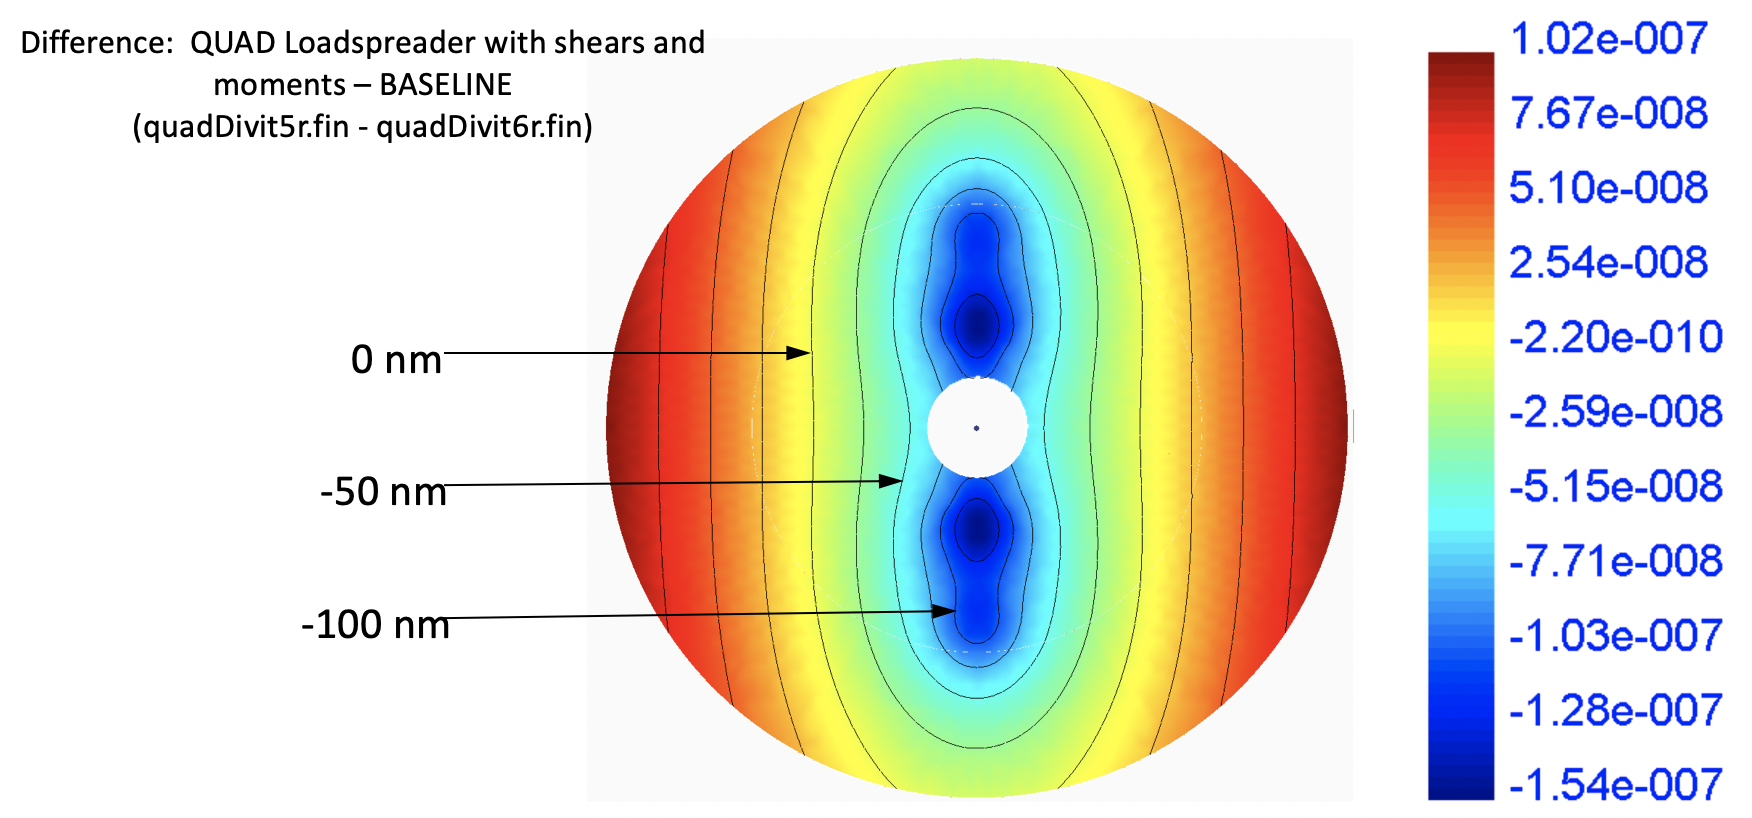
\includegraphics[width=140mm]{figures/divitsFEA.png}
  \end{tabular}
   \end{center}
   \caption
   { \label{fig:divitsFEA}
     FEA prediction of M1M3 surface shape due to shear forces and
     moments associated with the four quads.
 }
\end{figure}

Ideally, we would want to go back and change the load spreader design,
to avoid these unintended shear forces and moments.
However, given that the actuated tests have already been performed
using these hardware, and we've already achieved pretty good optimized
M1 and M3 surfaces, going back to change the design would invalidate
all the test results.
Changing the hardware design would also invalidate the single actuator
influence function measurements for the quads, and also bending modes,
to some extent.
We therefore choose to use the load spreaders and the actuators the
way they are.

 \subsection{Final Optimized Surfaces and Forces}
 \label{sec:optS}

 After understanding the root cause for the divits on top of the
 quads, it became obvious why we could not further improve the surfaces by
 adjusting actuator forces.
 
 As the final push for better surfaces, we ran another round of
 optimization on the last day of test campaign No. 2, by making a fit
 to the measured M1M3 surfaces using 14 single actuator influence
 functions.
 These 14 influence functions included the quads, their neighbor
 actuators on both sides in the $\pm$x direction, plus actuator
 No. 101 and 301.
 As expected, some small further improvements were achieved by
 adjusting these 14 actuator forces.
 After two iterations, the fit to the 14 influence functions yielded
 forces that were close to zero.

 
 Looking back at the entire surface optimization process, a few times
 we got to, or got close to, the best optimized M1 and M3 surfaces.
 \bitm
\item On 1/25, the last day of test campaign No. 1, using incorrectly
  calculated initial forces, Mirror Lab bending modes, and additional
  forces on the quads, we got to 33 and 28 nm RMS on M1 and M3,
  respectively. For historical reasons, we refer this force set as $f1$.
  \item On 2/14, the 4th day of test campaign No. 2, where we had
    started using the correct initial forces, and using LSST bending
    modes, with no additional forces on the quads, we reached 30 and
    26 nm RMS on M1 and M3,
    respectively. we refer this force set as $f3$.
    \item On 2/21, the last day of test campaign No. 2, for the final
      round of surface optimization, we started from $f3$. We call it
      iteration 0. For iteration 1, the surface RMS values were 28/24
      nm. We refer to this force set as $fa$. The force change between
      iteration 1 and 0 was up to $\sim$150 N, on the quads.
      \item On 2/21, for iteration 2, the surface RMS values were 31/20
      nm. We refer to this force set as $fb$. The force change between
      iteration 2 and 1 was up to $\sim$100 N, on the quads.
      \item On 2/21, for iteration 3, the surface RMS values were 27/21
      nm. We refer to this force set as $fc$. The force change between
      iteration 3 and 2 was up to $\sim$0.2 N, on the quads.
      \item On 2/21, by the end of the day, we measured the surfaces
        again by applying $fc$. Thermal conditions had drifted a bit
        by then. We reoptimized the M1 and M3 surfaces using 27 LSST
        bending modes. With 3 iterations, we got surface RMS values of
        28/20 nm. We refer to this force set as $fd$.
  \eitm

  The M1 and M3 surfaces, as produced by the above force sets, are
  shown in Figure~\ref{fig:optS}. The differences between them are small.
  These are also documented in
  \bitm
\item \url{https://github.com/bxin/M1M3_ML/blob/master/190125.ipynb}
\item \url{https://github.com/bxin/M1M3_ML/blob/master/190214.ipynb}
\item \url{https://github.com/bxin/M1M3_ML/blob/master/190221.ipynb}
  \eitm
  
 \begin{figure}[bthp]
   \begin{center}
     \begin{tabular}{c}
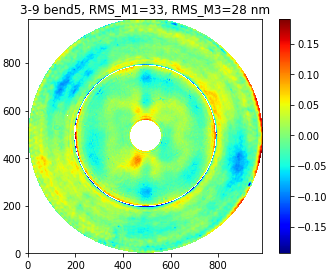
\includegraphics[width=50mm]{figures/optS1.png}
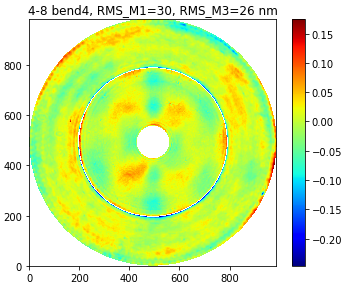
\includegraphics[width=50mm]{figures/optS3.png}
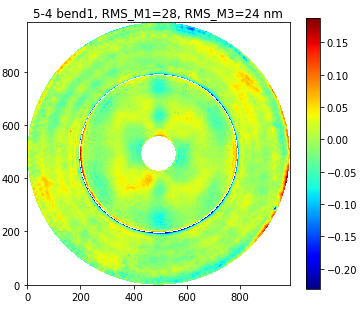
\includegraphics[width=50mm]{figures/optSa.png} \\
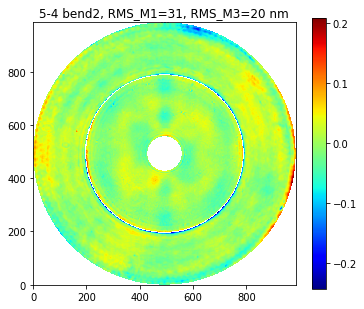
\includegraphics[width=50mm]{figures/optSb.png}
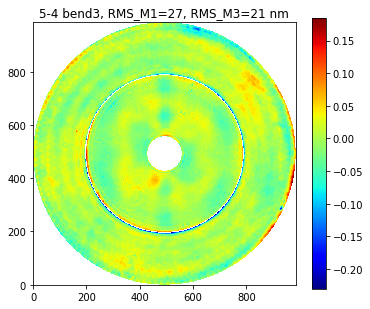
\includegraphics[width=50mm]{figures/optSc.png}
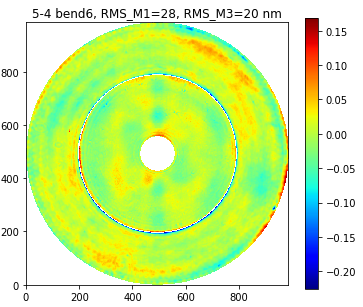
\includegraphics[width=50mm]{figures/optSd.png}

  \end{tabular}
   \end{center}
   \caption
   { \label{fig:optS}
     The M1 and M3 surfaces, as produced by force sets $f1$,
  $f3$, $fa$, (top row, from left to right), and $fb$, $fc$, $fd$
  (bottom row, from left to right).
 }
\end{figure}

 \subsection{M1M3 Structure function}

 See Figure~\ref{fig:SF} for the M1 and M3 structure functions (SF)
 calculated for the surfaces produced with the $fc$ force set above (27nm on M1 and 21nm on M3).
We also compare to three other curves as references:
 \bitm
\item The (2014) polishing specifications.
\item The SF for the 2014 polished surfaces.
  \item Revised (2019) specifications, by adding image quality
    allocations for temperature and force accuracy to the polishing
    specification. (note that we are using all the thermal allocation
    here: 54 mas for M1 and 54 mas for M3; and the 10 mas
    for force accuracy have been divided equally between M1 and M3. We
    left out the 10 mas budget for M1M3 vibration, since no cooling
    fans were installed).
    \eitm
For both mirrors we are meeting the SF specifications.
For M1, the SF increased pretty uniformly across the spectrum. This is true for both the specification curves and the measured SF. For M3, the increase in the measured SF is much more significant in the range roughly between 0.05m and 0.5m. At one point ($\sim$0.1m separation) it is basically touching the specification curve.

 
 \begin{figure}[bthp]
   \begin{center}
     \begin{tabular}{c}
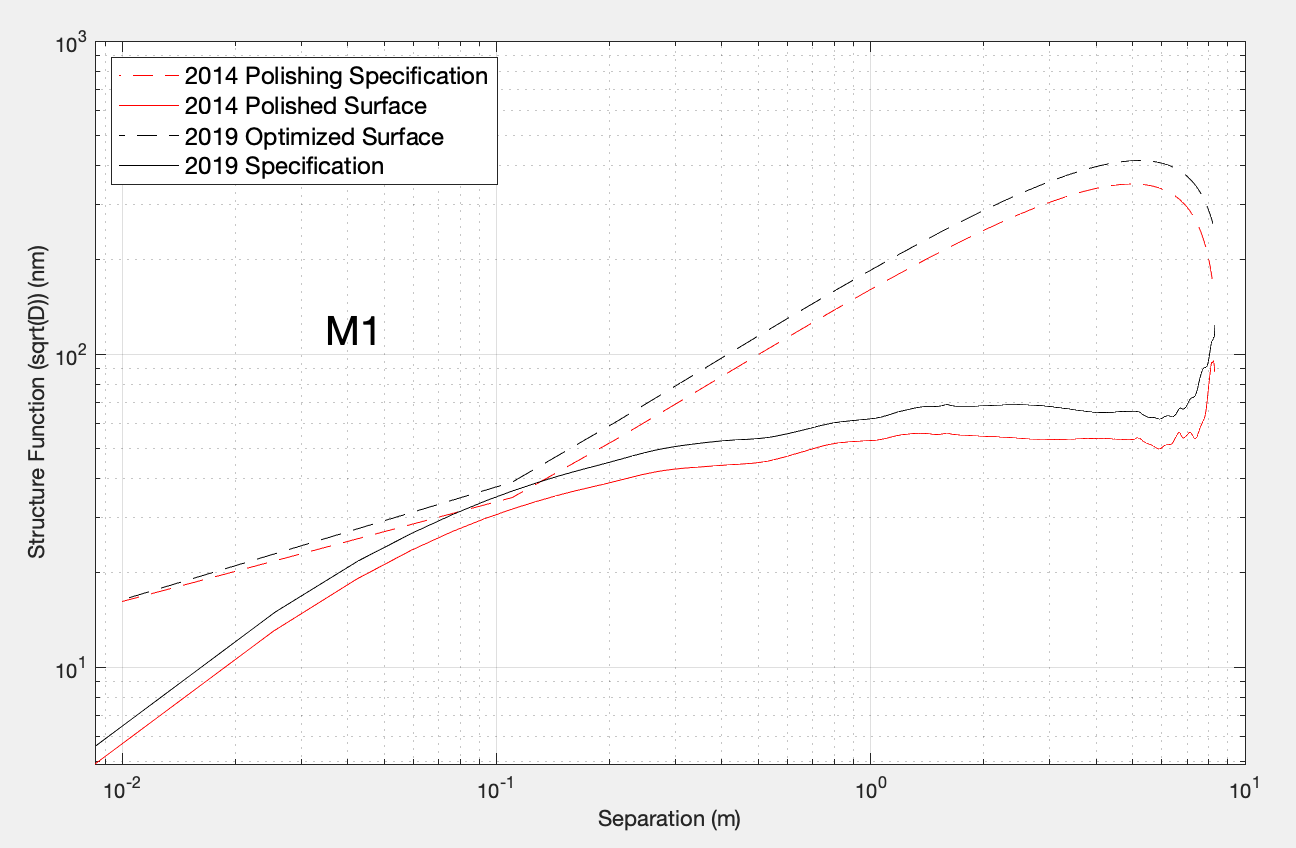
\includegraphics[width=140mm]{figures/M1SF.png}\\
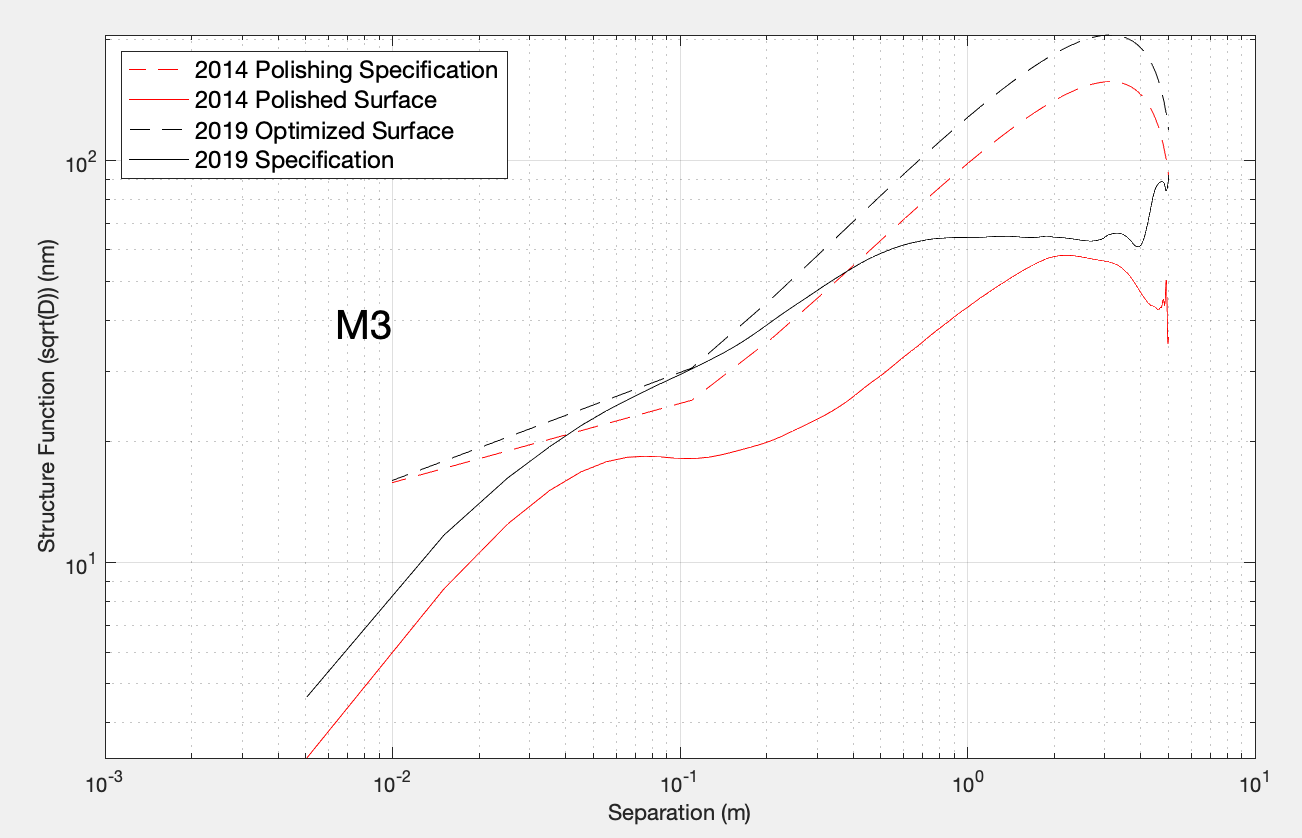
\includegraphics[width=140mm]{figures/M3SF.png}
  \end{tabular}
   \end{center}
   \caption
   { \label{fig:SF}
     The M1 and M3 structure functions, and comparisons to the 2014
     polished surfaces, and their corresponding specifications.
 }
\end{figure}
 
 \subsection{Image Quality Evaluation}

 We took the M1M3
 surfaces produced with the $fc$ force set above (27nm on M1 and
 21nm on M3), and inserted into the LSST optical design Zemax
 model (v3.3), to directly evaluate the impact of such a surface on
 the system image quality.
 The detailed procedure follows exactly what is decribed in
 document-17171~\cite{m1m3perf}.
 Wavefronts, in the form of 2048 $\times$ 2048 OPD maps, are evaluated
 at 31 Gaussian Quadrature (GQ) field points.
 These are then used to evaluate the Normalized Point Source
 Sensitivity (PSSN), changes in the 5$\sigma$ imaging depth ($\Delta
 m_5$), effective full-width at half maximum (FWHM), and FWHM.

The results for ideal optics with the $fc$ surfaces are shown in row
$q$ of Table~\ref{tab:fwhm}.
Rows $a$ and $g$ are copied from Document-17171~\cite{m1m3perf}.
We use $\Delta$ for the differences between the $fc$ surfaces and the
2014 polished M1M3 surfaces.
Polishing in 2014 was done on static supports.
Therefore, $\Delta$ has contributions from both the mirror surport
system and thermal factors.
When we do the subtraction between two rows, we take the ratio of the
PSSN values, then convert the resulting PSSN into $\Delta m_5$ and
effective FWHM ($FWHM_{\rm eff}$). 
The subtraction of FWHM is done by subtracting in quadrature.

The numbers in the parentheses are image quality budgets in FWHM.
For $\Delta$, these are actually the upper bonds.
The 77mas is the quadrature sum of 54mas (for M1 thermal), 54mas (for
M3 thermal), and the 10mas (for M1M3 actuator force accuracy).
Because further thermal FEA analyses were done after these budgets
were put in place, the current best knowledge is 69mas for M1 thermal
and 84mas for M3 thermal.
If we use these values then we get 109mas for the quadrature sum.
We left out the 10 mas budget for M1M3 vibration, since no cooling
    fans were installed.
    
\begin{table}[bpt]
%\small
%\footnotesize
\caption{Summary of PSSN,  $\Delta m_5$,  $FWHM_{\rm eff}$ and $FWHM$ for various
optical configurations of the M1M3. 
All numbers shown are GQ values across the 
31 field points as defined in Ref.~\cite{m1m3perf}.
The numbers in the the parentheses are image quality budgets in FWHM.}
%\tabcolsep=0.11cm
\vspace{1mm} \centering
\begin{tabular}{ll|cccc }\hline\hline
&& PSSN & $\Delta m_5$& $FWHM_{\rm eff}$ & $FWHM$ \\
& &  & (mmag)&(mas) &(mas)  \\\hline\hline
a&Ideal Optics &0.9787 & 12.0 & 96.1   & 100    \\
g&=M1M3 Polishing (no crows' feet) &0.9317  & 38.5 & 178.4 & 112 (112)  \\
q&=a+g+$\Delta$ & 0.9083  & 52.2  & 224.1 & 164 \\ \hline
  r& =g+$\Delta$ = q-a & 0.9137 & 49.1 & 200.3 & 129 \\
  $\Delta$ & = r-g & 0.9807 & 10.6 & 91.5 & 64 (77$|$109) \\
\hline
\hline
\end{tabular}
\label{tab:fwhm}
\end{table}

\subsection{Use of bending mode No. 27}

The test plan before the test campaigns started was to measure 22
bending modes. The surface optimization was also planned to be
performed using 22 bending modes.
However, during the surface optimization, it was observed at, when we
started with the calculated initial forces, we were often left with a
residual that looked like bending mode No. 27.
At that point we decided to include bending mode 27 in the surface
optimizations. And we measured bending modes up to No. 27, for both
the Mirror Lab bending modes and the LSST bending modes.

Now the question is,  
do we need bending mode 27 for AOS closed-loop?
Ref.~\cite{m1m3bm27} attempts to address this question, by looking through
the entire surface optimization - under what circumstances did we need
to include significant amount of bending mode 27 to improve the
surfaces.
The conclusion from Ref.~\cite{m1m3bm27} is that bending mode 27 was only
needed right after we started a round of surface optimization with
calculated initial forces. If the
starting force set already included bending mode 27, it won't be
needed for subsequent optimizations.
What that says is basically that we need bending mode 27 to go from
the initial calculated force set to the optimized force set. On top of
the optimized force set, additional environmental drift will not
require a correction with bending mode 27. In other words, bending
mode 27 is part of the static correction. It is not dynamic, and will
most likely not be needed during day-to-day AOS operations.

However, considering we have only been able to optimize the M1M3
surfaces at zenith, and when we go off-zenith, we would be mostly relying
on the FE model, we will include bending mode 27 in the AOS bending
modes.
Since the AOS software has been set up to use 20 M1M3 bending modes,
we will keep the total number to be 20. The actual set of bending
modes used will be 1-19, and 27.
Note that bending modes 19 and 20 are a symmetric pair, with $6\theta$
azimuthal dependence.
We do not measure $6\theta$ Zernikes terms ($Z_{27}$ and $Z_{28}$) with
our wavefront sensors anyway.
Bending mode 19 will likely not be used either, which we can easily
truncate off with the truncation of the optical sensitivity matrix.

\subsection{Building the LUT}
\label{sec:LUT}

In coming up with the LUT for zenith pointing, we want to average the
above force set, or a subset of them, so that we can average out
measurement noise to some extent.
Since $f1$ had additional forces on the quads, while others do not, it is not good to be
included in the average.
$f3$ was before we started optimizing using 14 influence functions, so
it is a bit different from the rest of the force sets. So we leave
that out as well.
$fa$ should not be included either because it is in the middle of
optimization with 14 influence functions, before things
completely converged.
$fb$ and $fc$ were after the convergence. There were literally no
difference between $fb$ and $fc$.
The difference between $fd$ and $(fb+fc)/2$ was a combination of the first
27 bending modes, actually dominated by the two astigma modes.
These were due to temperature drifts.
Considering that when we do this on the summit the temperate profile
will be different anyway, we take the average of $fb$, $fc$, and $fd$,
and use it as the final zenith-pointing LUT.
The analysis is documented in \url{https://github.com/bxin/M1M3_ML/blob/master/finalLUT.ipynb}.

To extend the LUT to off zenith, we need to combine the optimal forces
at zenith and those at horizon. The optimal forces at an arbituary
zenith angle $\theta_z$ has three components,
\beq
F = F_G(\theta_z) + F_B + F_a(\theta_z),
\label{eq:LUTF}
\eeq
where $F$ and each term on the right are 156$\times$1 vectors.
The first component $F_G$ is the force that is needed to counter
gravity of the glass mirror itself. It has a simple dependence on $\theta_z$.
\beq
F_G(\theta_z)  = F_{Gz} \cos \theta_z + F_{Gh} \sin \theta_z.
\eeq
The 2nd component is a static bending force.
The 3rd component is due to actuator weights, hence has a special
$\theta_z$ dependence, as shown in Eq. (19) and (20) of Ref.~\cite{m1m3initF}.

By doing this optical testing of M1M3 in the Mirror Lab, we know
$F_{Gz}$, $F_B$, and $F_a$. But since we did this at zenith only,
where $\sin\theta_z$=0, we couldn't learn anything about $F_{Gh}$,
hence the case for further horizon testing of M1M3 on the summit. For
horizon testing, we know $F_a(\theta_z = 90^\circ)$ and $F_B$, we will
be able to fine-tune $F_{Gz}$, by starting with the FEA-predicted
horizon forces. Note that the FEA-predicted horizon forces will
correspond to $F_{Gh} $, instead of $F$ in Equation~(\ref{eq:LUTF}), because the FEA
models a perfectly polished mirror, so there is no $F_B$ needed, and
the FEA doesn't know anything about $F_a$.

The notebook
\url{https://github.com/bxin/M1M3_ML/blob/master/get_Fxyz_from_EFD_190125.ipynb}
illustrates the different components of the forces at zenith, as
defined by the M1M3 control software, in the order they were added
during the testing,

\bnum [label=\Alph*]
\item 2014 polishing forces $-$ removed Mirror Lab hardware $+$
  installed LSST hardware;
\item forces due to lateral actuator weights;
  \item static bending modes needed in 2014 to theoretically bend
    the mirror into optimal shape;
    \item Force Balance (FB) forces for cancelling out any nonzero net
      forces and moments;
    \item Bending mode forces applied during optimization;
      \item Additional single actuator influence function forces applied during optimization.
\enum
Among these components, A is for countering gravity.
D is in principle due to gravity as well. But it is closely related
to the mirror as positioned relative to the mirror cell.
What we measured in the Mirror Lab
applied to the mirror positioning in the Mirror Lab. Considering that the
actuators are being reinstalled in Chile, and these forces are small,
and they will be reapplied automatically by the force balance system,
we leave them out in the LUT.
F is indirectly due to gravity - gravity requires large support forces
on the quads which leads to deformation of the load spreaders.
We expect F not to go to zero at horizon pointing, because there will
still be nonzero $F_z$ to stop the mirror from tipping over. But those
forces will be much smaller. And the nonzero effect will be taken into
account by $F_{Gh}$ when we do the optical testing at horizon.
\beq
F_G(\theta_z=0) = A+F.
\eeq
Obviously,
\beq
F_a(\theta_z=0) = B.
\eeq
C and E are about bending the mirror into optimal shape. Together
they make up
\beq
F_B = C+E.
\eeq

On the other hand, the M1M3 control software publishes the force
values and their components as part of the telemetry, at a frequency
of 50 Hz. These are captured by the 
EFD.
The relevant data tables are
\bitm
\item K1 = D = $m1m3\_logevent\_AppliedBalanceForces$
\item K2 = C = $m1m3\_logevent\_AppliedStaticForces$
\item K3 = E = $m1m3\_logevent\_AppliedActiveOpticForces$
\item K = A+B+C+D+E+F = $m1m3\_logevent\_AppliedForces$  or \\$m1m3\_logevent\_AppliedCylinderForces$  
  \eitm
  Therefore,
  \beq
  F_G(\theta_z=0) = A+F = K-B-C-D-E
  \eeq
  
The notebook
\url{https://github.com/bxin/M1M3_ML/blob/master/finalLUT.ipynb} shows
the numerical derivation of the LUT. The results are duplicated in
Figure~\ref{fig:LUT}. Once we've done the M3 horizon testing on the
summit, we will simply replace the FEA-predicted $F_{Gh}$ with
measured to get the updated LUT.


 \begin{figure}[bthp]
   \begin{center}
     \begin{tabular}{c}
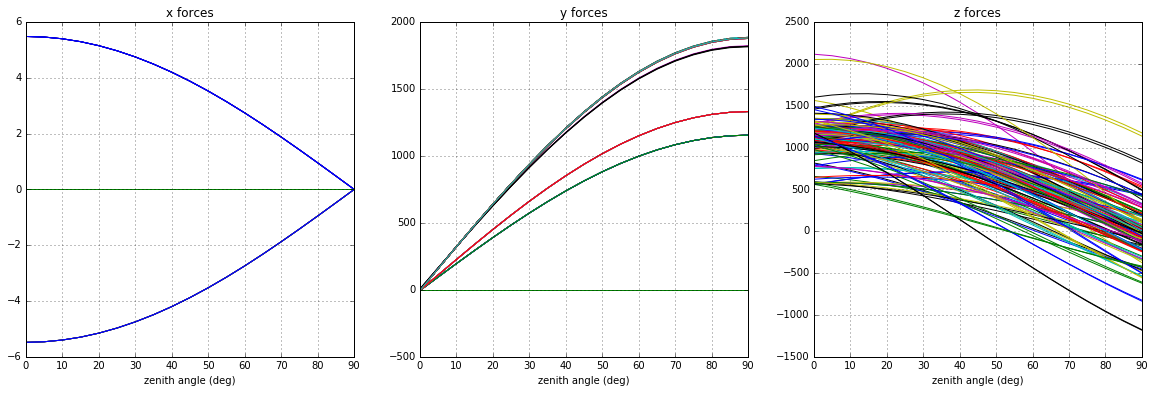
\includegraphics[width=170mm]{figures/LUT.png}
  \end{tabular}
   \end{center}
   \caption
   { \label{fig:LUT}
 The M1M3 LUT based on Mirror Lab test data at zenith pointing and FEA
 analysis at horizon pointing.
 }
\end{figure}

Document-34826~\cite{m1m3m2fbudget} gives the AOS force budget. For M1M3, this can be
summarized as
\bitm
\item The z-force has 4 components: Wavefront closed-loop (445N),
  slewing (150N), dynamics (5\% of total), and LUT (the rest);
\item The y-force has 3 components: slewing (400N), dynamics (5\% of
  total), and LUT (the rest);
  \item The x-force has 2 components: slewing (600N), dynamics (5\% of
    total). Yes, the remaining budget is unaccounted for. 
  \eitm
  We note that the forces calculated in this section all go into the
  ``rest'' category. For the x-forces, 
    Figure~\ref{fig:LUT} (left) shows we need nonzero, but small x
    forces in the LUT. The assumption is that these allocations are
    just guidelines, which will 
    not be strictly enforced by the control software. 
    Therefore, the x-force budget above does not have a LUT component.
    
\section{Horizon tests}
\label{sec:horizon}

Even though the testing at the Mirror Lab was only for zenith
pointing, we hoped to gain some knowledge about the mirror at horizon
pointing. As we discussed in Section~\ref{sec:LUT}, it is understood
that $F_{Gz}$ and $F_{Gh}$ are independent components, so we can not
simply learn about one and determine the other, however, there are two
things we could do at zenith pointing to help us get better informed
with the upcoming horizon testing on the summit. These are described in the
following two subsections.

\subsection{Horizon Bending Test}

 At horizon pointing, if we do not apply any axial force, i.e., let
 all $F_z$=0, then the mirror is going to sag.
The effect of applying the horizon optimized forces, $F_{Gh}$, is to
correct that sag. Without gravity pulling perpendicular to the optical
axis, the $F_{Gh}$ would produce a surface shape that is the inverse
of the horizon gravitational sag. So, we could apply the
FEA-determined $F_{Gh}$ in the Mirror Lab, measure the resulting
surface shape, then compare to FEA prediction.

Since the gravity is still going downward, this is essentially still a
bending test, i.e., these horizon forces we apply are nothing but a
particular combination of bending mode forces. We are not really
testing the behavior of the mirror at horizon pointing. Instead, we
are testing we can apply that particular force pattern, and see if it
produces a shape that resembles the FEA prediction.

There is still one subtlety here though. The horizon forces $F_{Gh}$
has a net $x$-moment. The reason is that the DAA pivoit points are on
a different $x-y$ plane from the center of gravity of the mirror. The
axial forces have to produce a net $x$-moment, to prevent the mirror
from tipping over.
Also note that, for simplicity, we decided to use only the axial
forces $F_z$ for mirror shape optimization. The lateral forces $F_y$ are only used
to support the mirror weight.

The details in deriving the horizon bending forces are found in Ref.~\cite{horizonFEA}. We provide a summary here.
\bitm
\item Ed Hileman provided a set of horizon forces, including $F_z$ and
  $F_y$. The $F_y$ forces, which are used to support the weight of the
  mirror at horizon pointing, came from some early Mirror Lab
  studies. They have a few discrete values, depending on the location
  and type of individual actuators.
On the other hand, the $F_z$ forces, although close to
being optimized, still needed further optimization.
Most likely Ed did the optimization early on using
  $z$-displacements. But these are just the starting point of our optimization. So it doesn't
  matter. We can converge to the optimal forces and surfaces with one correction.
  \item We applied the above forces in the latest M1M3 FEA model, at
    horizon pointing, and output the 3D displacements of each surface
    node.
    \item Surface normal displacements were calculated using the above
      3D displacements.
      \item We optimized the surface shape using the surface normal
        displacements together with the FEA surface normal bending
        modes. This gives us a set of optimized $F_z$ and the
        optimized surface shape it produces, when combined with the
        $F_y$ which has been fixed.
        \item The above optimized forces were applied to the FEA
          model, so that we could output the 3D displacment vectors,
          calculate the surface normal shape, and compare to the
          optimized shape calculated above. This step is just a sanity
          check.
        \item Make a linear fit to the optimized $F_z$,
          \beq
          F_z = b y
          \eeq
          Then subtract $by$ from $F_z$
          \item Verify that the new $F_z$ satisfies $\sum(F_z)$=0,
            $M_x$=0, and $M_y$=0.
            \item Determine the surface change that is produced by
              this force set using the FEA, i.e., determine zenith
              optimized forces and surface shape first, then add the
              balanced $F_z$ forces from above, take the difference
              between the two set of 3D displacment vectors, convert
              to surface normal shape, and subtract PTT separately
              from M1 and M3. Alternatively, this step can be achieved outside of the
              FE model using the full influence matrix of the mirror.
              \item Based on the predicted force map and surface
                change, determine a scale factor to be used in Mirror
                Lab testing. (A surface RMS around 500nm is easist to
                measure by the interferometers). The scale factor was
                determined to be 1/4.
                \item Apply the scaled forces in the Mirror Lab,
                  make the M1-M3-M1 measurements before and after applying these
                  additional forces. Take the difference, apply the
                  invert of the scale factor, i.e., multiple by 4, compare to
                  the FEA prediction.
                  \item Fit the measured horizon bending shape to the
                    FEA predicted shape. Obtain the scaling factor
                    between measured and the FEA, and the residual map.
\eitm

Figure~\ref{fig:horizonS} shows results from this test.
The measured horizon bending shape and the FEA-predicted horizon
bending shape are shown. After making the fit to the measured horizon
shape using the FEA 
predicted shape, the scaling factor, which is the ratio between
measured and FEA prediction, was found to be 1.039.
Note that this shape is largely made of coma, i.e., bending mode
No. 7. For earlier results, the scaling factor for bending mode No. 7
was found to be 1.032. 

 \begin{figure}[bthp]
   \begin{center}
     \begin{tabular}{c}
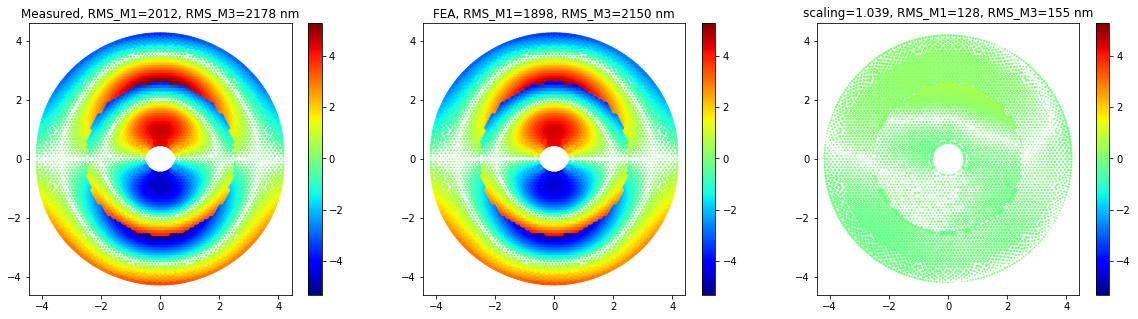
\includegraphics[width=170mm]{figures/horizonS.png}
  \end{tabular}
   \end{center}
   \caption
   { \label{fig:horizonS}
Results of horizon bending test. Left: measured horizon bending shape
interpolated onto FEA grid,
Center: FEA-predicted horizon bending shape, and Right: residual map
from making a fit to the measured horizon shape using the FEA
predicted shape. The scaling factor, which is the ratio between
measured and FEA prediction, is found to be 1.039.
 }
\end{figure}


  \subsection{Inferring M1 shape from M3 measurements}
  
For M1M3 horizon test on the summit, the plan has always been to test
M3 only, because M1 radius of curvature will not be accessible.
However, the horizon optimized forces $F_{Gh}$ should optimize M1 and
M3 surfaces simultaneously. So the question is, can we optimize M1 and
M3 surfaces at the same time while we can only measure M3 shape? i.e., how
well can we know M1 shape based on M3 measurements?
As of the time this note is written, it looks unlikely that we will
measure M3 interferometrically on the summit, due to potential
challenges with interferometer alignment and amount of mechanical
engineering work needed to put up the hardware. Instead, a
Shack-Hartmann test for measuring M3 surface is being planned.

To answer the above question, the key is to realize that, what enables
us to relate M1 surface with M3 surface is the fact that they are on
one substrate, i.e., there is one set of forces.
In the absense of measurement noise (on both the surface shape and the
forces), any actuator under M1 can produce a noticeable shape change
on M3, and vice versa. In that case, using M3 surface measurement, we
can perfectly derive all the actuator forces. Multiplying that with the
full mirror influence function gives of shapes of both M1 and M3.

But problems arise when there is noise.
The forces for those actuators under M1 can be not accurately
estimated using M3 surface measurement.
The high spatial frequency
components in the global M1M3 surface shape can not be inferred from
M3 measurements alone.
To suppress noise, we have to leave out the high frequency components
on M3.
The math, the results, and the numerical analyses are documented in
Document-32377~\cite{inferm1p1} and 32378~\cite{inferm1p2}.
The basic conclusion was that
inferring M1 shape from M3 measurements works for low order bending modes ($\sim<$15), not high order one.

As documented in \url{https://github.com/bxin/M1M3_ML/blob/master/190221.ipynb},
in the Mirror Lab, we started with 500nm of horizon deformation (about
1/4 of the inverse of the horizon gravitational sag), which is largely
y-coma, and by keeping the first 15 singular values in the SVD the M3-only
influence matrix, we reduced it by a factor of 3 (to 174nm) by optimizing M3
only.
The 174nm comes from two sources.
\bnum
\item One is that inferring M1 from M3 measurements simply does not work for the high order modes.
Analysis shows that in the measured horizon test surfaces, the
root-sum-square (RSS) of the high order modes ($>15$) accounts
for 148nm out of the 174nm of the total surface RMS.
We know we cannot correct that. Modes 1-15
gives 481nm.
$\sqrt{481^2+148^2}=500$nm.
The high spatial order components are simply there, and we know we
cannot do anything about it. So we choose to 
 filter out the high order modes with data processing, specifically,
 when we try to infer all 156 forces using M3 measurements.
\item
The other is the bending modes we use for this M1 prediction are FEA
bending modes, which is different from the real mirror bending modes.
\enum
There are other sources as well, such as temperature drifts between
the iterations, and measurement noise, which should be much smaller
than 1 and 2 above. By filtering out the high order modes, we can
largely avoid the amplification of the measurement nose, but there is
no clean cut.

So if we do this on the summit, we will start from FEA predicted
horizon forces. Without any axial force optimization we have 2 microns
of surface deformation. If we assume 90\% FEA accuracy, we will be off
to $\sim$200nm. If we still reduce it by a factor of 3, we get to
$\sim$70nm.
We will not be able to reduce or eliminate item 2 above, because as
we discussed in Section~\ref{sec:optS}, we will use the bending mode
shapes as they are derived from the FE analysis.

Since we only correct low order modes, we do not really need the high
spatial resolution provided by the interferometer. In that sense, a SH
would be good enough. 

\section{Actuator Force Error}
\label{sec:ferror}

Using the telemetry data collected during these tests, we have also
been able to look at the difference between the applied forces and the
measured forces.
The applied forces are the forces as given by the force commands,
found in the EFD table $m1m3\_logevent\_AppliedForces$.
The measured forces are what the load cells tell us that has been
applied, found in the EFD table $m1m3\_ForceActuatorData$.
The difference between the two reflects the ILC's ability to reach the
target force values. For example, there may be a lack of air pressure, problems
with the control valves, or just simply a glass safty limit.

In the analysis documented by
\url{https://github.com/bxin/M1M3_ML/blob/master/ForceError.ipynb},
we looked at actuator force differences within three 4-minute
periods. These were from three different days during test campaign
No. 1.
The three days are at the beginning, middle, and end of the test
campaign.
Ideally we would also pick some dates from test campaign No. 2. But
problems with unintended data truncation in the EFD prevented us from
doing that. More details are explained in the above notebook.
We took three time stamps, each associated with some other
measurements, as found in the per-day activities notebooks, and
selected data within $\pm$2 minutes of those time stamps.
The telemetry data was taken at frequency of 50 Hz. But there are some
data missing in the EFD. So while taking the difference between the
two sets of forces, we averaged each set of forces within 1-second time intervals.
Another subtle thing here is that the database query has to be done
using time stamps that the data was recorded in the EFD, which is in
sequential order. When we match the two sets of forces, we had to use
the time stamps when the telemetry messages were sent, which are not
in sequential order sometimes, and therefore couldn't be used in the
database query.

Figure~\ref{fig:forceError} shows the force differences in their x, y,
and z-components. Each entry in the histograms is a force difference
for one actuator within a particular 1 second.
The x and y force errors are basically negligible (compared to the
force error requirement as shown in LTS-88~\cite{lts88} Table 3).
The z force errors can be as large as 2N, which may require some attention.
It is clear that the force error statistics is not drifting over time, i.e.,
this is repeatable over the entire period of test campaign No. 1.

 \begin{figure}[bthp]
   \begin{center}
     \begin{tabular}{c}
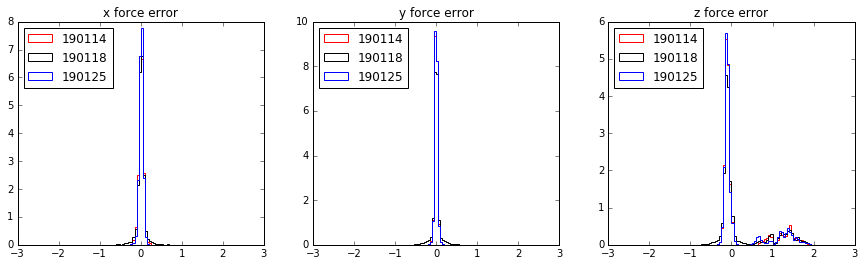
\includegraphics[width=170mm]{figures/forceError.png}
  \end{tabular}
   \end{center}
   \caption
   { \label{fig:forceError}
Actuator force error distributions within three 4-minute periods from
different days during test campaign No. 1. For comparison purpose, each histogram is
normalized to total area of 1.
 }
\end{figure}

Then the next question is, do the force errors vary by actuator? i.e.,
for a particular actuator, does it always have the same force error?
To answer that question, we looked at the same kind of histograms,
like those shown in Figure~\ref{fig:forceError}, by actuator.
There are too many (N=156, for the z-forces) such histograms. We do not
reproduce them here. Instead, the reader is referred to the notebook
\url{https://github.com/bxin/M1M3_ML/blob/master/ForceError.ipynb}.
The conclusion there is that, indeed, the force errors for individual
actuators are mostly repeatable. The non-repeatable errors, as shown
by the width of the histograms, are negligible. LTS-88~\cite{lts88}
has the requirements on the
non-repeating errors of the order $\sim$0.5N.
The repeatable force errors are as large as $\sim$2N, but still
well below those required by LTS-88~\cite{lts88}  Table 3, which is 4.45N for x, y,
and z forces.

We took the average of the per-actuator force error histograms, and
produced a force offset table (found in the github repo, $data/$
folder). We plan to add these systematic offsets to the control
software, so that when force commands are sent out, these are already
taken into account.

Note that this is separate from the calibration of
the actuator load cells. If the load cells are not sufficiently calibrated,
there could be errors and biases in the load cell reading. That could
be an additional source of the force error.
This calibration has been discussed in Section~\ref{sec:divits}.
The repeatable part of these force errors can also be easily taken out
using the control software. Even if that is not done, they will
largely be taken out by the AOS.
It is the non-repeatable force error, which changes randomly with
time, that could be more problematic.
To the first order, they would produce nothing but astigmatisms on the mirror
surfaces.

According to document-20263~\cite{m1m3faccuracy}, 0.5N non-repeating force errors produce
about 5 mas of image degradation in effective FWHM.
LTS-123~\cite{lts123} and 124~\cite{lts124} have the image quality allocation to M1M3 actuator
force error as 10 mas. So we are well within the image quality budget
here.
Systematic calibration of all the load cells will allow us to further
determine whether the contribution from actuator force errors is
indeed below its image quality allocation.

\section{Performance of the EFD}
\label{sec:efd}

As we pointed out in Section~\ref{sec:intro}, the performance of the
EFD left a lot to be improved.
While the EFD was 
supposed to capture all the telemetry, events, and commands as
published by the M1M3 control software,
the actual performance, as indicated by the the capturing rate of the
telemetry events, is shown in Figure~\ref{fig:efd}.
The absolute normalization of the y-axes is arbituary due to histogram
binning - each point covers 10 minutes time interval.
In each case, the maximum of the y-ranges corresponds to telemetry
capturing rate of 1.
The M1M3 control system publishes telemetry at 50 Hz.
The thermal data was published once a minute.

 \begin{figure}[bthp]
   \begin{center}
     \begin{tabular}{c}
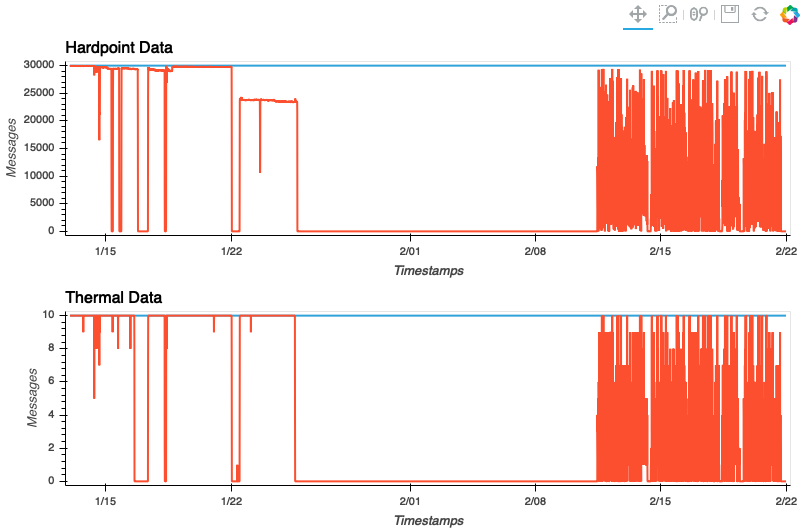
\includegraphics[width=170mm]{figures/EFD_messages_both_campaigns.png}
  \end{tabular}
   \end{center}
   \caption
   { \label{fig:efd}
Some telemetry event rates as a function of time. The time range in
these plots covers both test campaigns. Plots made by Michael Reuter.
 }
\end{figure}


This version of the EFD, based on MariaDB, instead of the InfluxDB
which will be used for final versions of the LSST EFD, worked $\sim$
80\% of the time during campaign No. 1.
During campaign No. 2 the capturing rate has been much worse, as seen
in Figure~\ref{fig:efd}.
This is in addition to the force value truncation problem as we
mentioned in Section~\ref{sec:ferror}.


\section{Summary}

Overall, the M1M3 optical testing at the UofA Mirror Lab has been a
great success. We encountered some challenges along the way, mostly
with surface optimization, but in the end we solved all the problems
by understanding their causes, and we achieved the major goals of the
testing campaigns. The only unachieved task as outlined in the test
plan was to measure vibration when the cooling fans are turned
on. This was not done due to problems turning on the cooling fans. But
this was designed as an optional test from the very beginning.

These testing campaigns are the 
first step in building up our understanding of the entire LSST optical system.
Once the system is reassembled in Chile, with the surrogate mirror
instead of the real glass mirror, a portion of these tests will be
repeated on the summit.
After we do the M3 testing on the summit, we will update the LUT by
replacing the horizon FEA-determined optimal forces with the measured
optimal forces. Then the M1M3 LUT will be ready to go on sky with the
three-mirror system.

\bibliographystyle{spiebib}
\bibliography{report}   %>>>> bibliography data in report.bib

\end{document}
